\documentclass[11pt]{amsart}
\usepackage{geometry}                % See geometry.pdf to learn the layout options. There are lots.
\geometry{letterpaper}                   % ... or a4paper or a5paper or ... 
%\geometry{landscape}                % Activate for for rotated page geometry
%\usepackage[parfill]{parskip}    % Activate to begin paragraphs with an empty line rather than an indent
\usepackage{graphicx}
\usepackage{amssymb}
\usepackage{lscape}
\usepackage{booktabs}
\usepackage{caption}
\usepackage{longtable}
\usepackage{epstopdf}
\usepackage{verbatim}
\usepackage{rotating}
\usepackage{multirow}
\usepackage{multicol}
\usepackage{booktabs}
\usepackage{subfigure}

\usepackage{algorithm}
\usepackage{algpseudocode}
\DeclareGraphicsRule{.tif}{png}{.png}{`convert #1 `dirname #1`/`basename #1 .tif`.png}
\newtheorem{proposition}{Proposition}
\newtheorem{definition}{Definition}
\newcommand{\vertgeq}{\rotatebox{90}{$\leq$}}
\newcommand{\vertg}{\rotatebox{90}{$>$}}
\title{Draft}
\author{Lapo Santi}
%\date{}                                           % Activate to display a given date or no date

\begin{document}
\maketitle
%\section{}
%\subsection{}
\tableofcontents

\newpage

\section{Introduction}



When faced with a multitude of alternatives, individuals often strive to organize them into coherent blocks or groups to better understand the decision landscape. Furthermore, they aim to establish a meaningful order within these blocks, enabling them to prioritize alternatives based on preference. This process involves two fundamental tasks: block clustering and order-based ranking. While clustering involves categorizing alternatives into distinct blocks, ranking focuses on arranging these blocks in a specific order. These tasks are typically accomplished through human judgments, often in the form of pairwise comparisons.

In block clustering, the aim is to determine the inherent similarities among alternatives and group them accordingly. By comparing pairs of alternatives, individuals can identify common characteristics, shared attributes, or comparable features that contribute to their clustering. This process helps unveil the underlying structure of the alternatives, allowing decision-makers to comprehend the relationships and associations between them. Several techniques, such as hierarchical clustering and k-means clustering, have been employed to address this task effectively.

Conversely, in order-based ranking, the primary objective is to establish a preference-based order among the identified blocks of alternatives. By comparing pairs of blocks, individuals can discern the relative favorability of one block over another. These pairwise comparisons generate a ranking list that encapsulates the perceived preference or priority of each block. Various methodologies, including the Bradley-Terry model and pairwise comparison matrices, have been utilized to derive meaningful rankings from the collected preferences.

In this article, we propose a novel approach, termed Block Clustering and Order-based Ranking (BCOR), which unifies the tasks of block clustering and order-based ranking into a cohesive framework. The BCOR model introduces a dynamic parameter that governs the granularity of block clustering, allowing decision-makers to explore a spectrum of clustering options. By iteratively adjusting this parameter, the model can encompass a wide range of decision-making scenarios, from finely differentiated blocks to coarser groupings.

A key insight of the BCOR model lies in its ability to relate the number of blocks to the underlying ranking structure. As the number of blocks converges to the total number of alternatives, the model effectively transitions into a traditional ranking approach, providing a complete ordering of the alternatives. Conversely, by intentionally reducing the number of blocks, decision-makers are presented with distinct groups of choices, each requiring preference considerations within its own subset. This approach offers a nuanced perspective on decision-making, allowing individuals to differentiate between highly favored groups and those that are comparatively less preferred.

The BCOR model provides a flexible and adaptive solution for organizing and prioritizing alternatives in various decision-making contexts. Its application extends beyond conventional clustering and ranking tasks, empowering decision-makers to explore the continuum between comprehensive rankings and granular groupings. Additionally, the model can be tailored to incorporate different types of pairwise comparisons, enabling its utilization in diverse domains and decision scenarios.

To evaluate the effectiveness of the BCOR model, we conducted experiments using real-world datasets encompassing a wide range of decision contexts. The results demonstrate the model's ability to generate meaningful block clusters and order-based rankings, outperforming traditional approaches that solely focus on clustering or ranking tasks.

The contributions of this work can be summarized as follows:

We introduce the novel problem of block clustering and order-based ranking, bridging the gap between these two fundamental decision tasks.
We propose the BCOR model, which provides a unified framework to accommodate various levels of granularity in decision-making, from complete rankings to distinct preference-based groups.
We showcase the versatility of the BCOR model through experiments on real-world datasets, highlighting its superior performance compared to existing methods.
By integrating block clustering and order-based ranking, the BCOR model offers decision-makers a comprehensive tool to navigate complex decision landscapes

\section{The simple model}

\subsection{Simple Model specification}

This is a model for pairwise count data. We explicitly model the results of the interactions between two individuals $i$ and $j$. Given $N$ observations, the likelihood is 
\begin{align}
p(y| z, P, K) &= \prod_{i =2 }^{N-1} \prod_{j =i}^{N} p(y_{ij} | z, P, K) \\ 
&= \prod_{i =2 }^{N-1} \prod_{j =i}^{N}  {n_{ij} \choose y_{ij}} p_{z_i, z_j}^{y_{ij}}(1- p_{z_i, z_j})^{n_{ij}-y_{ij}}
\end{align}

where $n_{ij}$ denotes the total number of interactions between the two individuals $i$ and $j$ and $y_{ij}$ is the number of successes of the individual $i$ in interacting with $j$. The probability of success is given by $p_{z_i, z_j}$ which consists of two parameters. The $K\times K$ matrix $P$ and the $N \times 1$ vector $z$.

The vector $z$ has entries $z_i$ taking values over the discrete and finite set $\{ 1 , \ldots, K\}$, and it is an indicator variable such that if $z_i = k$ individual $i$ belongs to block $k$. 

The matrix $P$ contains the probabilities of success for individuals belonging to each possible blocks combination. For this reason $P$ is $K\times K$. Therefore, the parameter $p_{z_i, z_j}$ consists in the probability of success in an interaction between one individual belonging to block $z_i$ and another of block $z_j$. 

\subsection{Prior Specification}


Starting with the parameter $P$, we assume that its entries, namely $p_{k,k^\prime}$, are independent and identically $Beta(a,b)$ distributed random variable. By setting $a=b=1$ they collapse to a uniform distribution.
\begin{equation}
p_{k,k^\prime} \sim Beta(1,1) \quad \text{for } k,k^\prime = 1, \ldots,K
\end{equation}
Second, we assume that the $z_i$s are independent and identically drawn from a multinomial distribution with one trial and probability vector $(\theta_1, \dots, \theta_K)$. We can write then:
\begin{equation}
z_i| \boldsymbol{\theta} \sim \operatorname{Multinomial}(1,\boldsymbol{\theta}) \quad \text{for } i = 1, \ldots,N
\end{equation}


To have more flexibility in the blocks sizes, we put an hyper-prior on the $\theta_1, \dots, \theta_K$, assuming that they are drawn from a Dirichlet distribution with parameter the $K\times1$ vector $\boldsymbol{\gamma}$.


By marginalizing out $\theta$, following the common practice in the literature, we can express the marginal distribution of $z$ as:

\begin{equation} p(\mathbf{z}|\boldsymbol{\gamma}) = \frac{\Gamma(\sum_{k=1}^K \gamma_k)}{\prod_{k=1}^K \Gamma(\gamma_k)}\frac{\prod_{k=1}^K \Gamma(n_k+\gamma_k)}{\Gamma(\sum_{k=1}^K (n_k+\gamma_k)}
\end{equation}

where $n_k$ is the number of players assigned to block $k$.

Finally, we assume that the number of clusters $K$ follow a Poisson distribution $\operatorname{Poisson}(\lambda=1)$, subject to the condition $K>0$.

\section{Connection with Image Recognition}

By drawing inspiration from the literature in Image Recognition, in particular an article of Noel Cressie and Jennifer Davidson, we represent our matrix $P$ as if it was an image, its probabilities as if they were pixels of different intensities, and its entries' indices as if they were pixels' locations. 

Let us denote a generic entry of $P$ as a vector $s$ in $\mathbb{N}^2$. The quantity $Z(s)$ denotes the probability value at the entry index $s$. We rewrite the whole matrix as 
\begin{equation}
Z = \{Z(s): s \in D \}
\end{equation}
where $D$ is the set of entries' indices of the matrix $P$, that is:
\begin{equation}
D = \{(u,v): u = 1,\ldots,K;v=1,\ldots,K\}.
\end{equation}

Now, let us consider a temporal Markov process \{Z(t): t=1,2,\ldots\}. The Markov property can be generalised from a one-dimensional time-process to a two-dimensional space with both a conditional and a joint specification. 

We draw a connection between the class of models called Partially Ordered Markov models which allows us to efficiently compute the joint probabilities of the prior on $P$, and the literature on preference learning.

Then we introduce the notion of partial order among the $P$ entries. Let's take once more $D$. The binary relation $\succeq$ on $D$ is said to be a partial order if 
For any $x \in D, x \prec x$ (reflexivity).
For any $x, y, z \in D, x \prec y$ and $y \prec z$ implies $x \prec z$ (transitivit
y).
For any $x, y \in D, x \prec y$ and $y \prec x$ implies $x=y$ (antisymmetry).
Then we call $(D, \prec)$ a partially ordered set, or a poset. For example, the set of all subsets of a given set, with the relation $\prec$ being set inclusion, is a poset.

Regarding the matrix $P$, we can check whether and how to use the definition of Poset under the three different axiomatic frameworks that specify different (stochastic) transitivity requirements.

\begin{enumerate}
\item Weak Stochastic Transitivity (WST): $\mathbb{P}(x \prec y) \geq \frac{1}{2}$ and $\mathbb{P}(y \prec z) \geq \frac{1}{2}$ imply $\mathbb{P}(x \prec z) \geq \frac{1}{2}$, for all $x, y, z \in \mathcal{A}$.

\item Strong Stochastic Transitivity (SST): $\mathbb{P}(x \prec y) \geq \frac{1}{2}$ and $\mathbb{P}(y \prec z) \geq \frac{1}{2}$ imply $\mathbb{P}(x \prec z) \geq \max \{\mathbb{P}(x \prec y), \mathbb{P}(y \prec z)\}$, for all $x, y, z \in \mathcal{A}$.

\item Linear Stochastic Transitivity (LST): $\mathbb{P}(a \prec b) = F(\mu(a) - \mu(b))$ for all $a, b \in \mathcal{A}$, where $F:\mathbb{R} \to [0, 1]$ is an increasing and symmetric function (referred to as a "comparison function"), and $\mu: \mathcal{A} \to \mathbb{R}$ is a mapping from the set $\mathcal{A}$ of alternatives to the real line (referred to as a "merit function").
\end{enumerate}

Each of these axioms, produces a different $P$ structure. Assuming, without loss of generality, that block 1 is the strongest, and by imposing the main diagonal to be equal to $\frac{1}{2}$ we can visualise a matrix following WST as:

\begin{center}
\begin{equation}
\label{eq:WST_P}
P^{WST} = 
\left(\begin{array}{cccc}p_{1,1} & p_{1,2} &  ... & p_{1,K} \\ p_{2,1} & p_{2,2} & ... & p_{2,K} \\ \vdots & \vdots & \vdots & \vdots \\ p_{K,1}& p_{K,2 }& ... & p_{K,K}\end{array}\right) =  
\left(\begin{array}{cccc} 1/2 \leq & p_{1,2} & ... & p_{1,K} \\  p_{2,1} \leq &  1/2 \leq & ... &  p_{2,K}  \\ \vdots & \vdots & \vdots & \vdots \\  p_{K,1}& p_{K,2 }&  ... &  1/2 \end{array}\right) 
\end{equation}
\end{center}
 
Instead, under SST, we would observe:
\begin{center}
\begin{equation}
\label{eq:SST_P}
P^{SST} = 
\left(\begin{array}{cccc}p_{1,1} & p_{1,2} &  ... & p_{1,K} \\ p_{2,1} & p_{2,2} & ... & p_{2,K} \\ \vdots & \vdots & \vdots & \vdots \\ p_{K,1}& p_{K,2 }& ... & p_{K,K}\end{array}\right) =  
\left(\begin{array}{cccc} 1/2 \leq & p_{1,2}\leq &  ... &  p_{1,K}  \\ \vertgeq &  \vertgeq &  & \vertgeq \\
 p_{2,1} \leq & 1/2 & ... & \leq p_{2,K} \\ \vdots & \vdots & \vdots & \vdots \\ p_{K,1} \leq & p_{K,2 } \leq & ... & \leq 1/2 \end{array}\right)  
 \end{equation} 
\end{center}


With regard of $LST$, it is a generalisation of the two axioms and therefore it includes both aforementioned cases \eqref{eq:WST_P} and \eqref{eq:SST_P}, depending how one specifies $F$ and $\mu$. Given the $LST$ definition, we can calculate $p_{ij}$ as follows:
\begin{equation}
p_{ij} = F(\mu(i) - \mu(j))
\end{equation}
where $i$ and $j$ range from 1 to $K$ and represent the alternatives in the set $\mathcal{A}$.

All the three axiomatic frameworks satisfy (in the $LST$ case we need to check the functional form of $F$ and $\mu$) of the three conditions for being a poset. And therefore, we take advantage of the poset structure.



We can now describe the correspondence referred to above. This connection opens up a large literature on graphical models, outside of statistical image analysis, that we return to in Section 6.2. Let $(D, F)$ be a directed acyclic graph, where $D=$ $\left\{y_1, \ldots, y_n\right\}$, a finite set. To construct a poset to which this digraph corresponds, we define the binary relation $\prec$ on $D$ by
$$
\begin{aligned}
& y_i \prec y_i, \text { for } i=1, \ldots, n \text {; } \\
& y_i \prec y_j, \text { if there exists a directed path from } y_i \text { to } y_j \text { in }(D, F) .
\end{aligned}
$$
Notice that several different directed acyclic graphs can yield the same poset.
Conversely, given a finite poset $(D, \prec)$, a corresponding directed acyclic graph can be obtained by defining the set of edges $F$ as follows:
$\left(y_i, y_i\right) \in F$ if and only if $y_i \prec y_j$ and there does not exist a third element
$$
z \neq y_i, y_j \text { such that } y_i \prec z \prec y_j \text {. }
$$
We saw above that the correspondence is many-to-one. Given a finite poset, one may construct a class of directed acyclic graphs; the correspondence described above is in a sense the minimal directed acyclic graph since it has the smallest possible directed edge set. However, if one starts with a directed acyclic graph, the corresponding poset is unique. From the point of view of image modeling, we arc more interested in the directed-acyclic-graph description because we are able to specify directly the spatial relations between pixel locations.



\section{The SST model}


We consider a Partially Ordered Markov Model (POMM) for a set of entries $p_{ij} \in L^{(k)}$, where $L^{(k)}$ represents a level set. These entries are assumed to be identically and independently distributed according to a truncated normal distribution:

\[
p_{ij}^{(k)} \mid (y^{(k)}, y^{(k+1)}) \sim \text{TruncatedNormal}(\mu^{(k)}, \sigma^{2(k)}; 0.5, \beta_{\max})
\]

The full prior is given by:
\[
p(P) = \prod_{k=1}^K \frac{1}{\sigma} \frac{\frac{1}{\sqrt{2\pi}} e^{-\frac{1}{2}\left(\frac{p_{ij} - \mu}{\sigma}\right)^2}}{\int_{-\infty}^\beta \frac{1}{\sigma\sqrt{2\pi}} e^{-\frac{1}{2}\left(\frac{t- \mu}{\sigma}\right)^2 }dt -\int_{-\infty}^{0.5} \frac{1}{\sigma\sqrt{2\pi}} e^{-\frac{1}{2}\left(\frac{t- \mu}{\sigma}\right)^2 }dt}
\]
Here:
\begin{itemize}
\item $\mu^{(k)}$ is the mean, which corresponds to the midpoint of the level set $L^{(k)}$, defined as $\mu^{(k)} = \frac{y^{(k)}+y^{(k+1)}}{2}$.
\item $\sigma^{2}$ is the variance parameter constant across the level sets $L^{(1)},\ldots,L^{(K)}$.
\item $0.5$ and $\beta_{\max}$ are the lower and upper truncation bounds.
\end{itemize}

It is interesting to see what happens when $\sigma \rightarrow \infty$
\begin{align}
&\lim_{\sigma \rightarrow \infty} \frac{1}{\sigma} \frac{\frac{1}{\sqrt{2\pi}} e^{-\frac{1}{2}\left(\frac{p_{ij} - \mu^{(k)}}{\sigma}\right)^2}}{\int_{-\infty}^\beta \frac{1}{\sigma\sqrt{2\pi}} e^{-\frac{1}{2}\left(\frac{t- \mu^{(k)}}{\sigma}\right)^2 }dt -\int_{-\infty}^{0.5} \frac{1}{\sigma\sqrt{2\pi}} e^{-\frac{1}{2}\left(\frac{t- \mu^{(k)}}{\sigma}\right)^2 }dt} = \\
&\lim_{\sigma \rightarrow \infty} \frac{1}{\sigma} \frac{\frac{1}{\sqrt{2\pi}} e^{-\frac{1}{2}\left(\frac{p_{ij} -  \frac{y^{(k)}+y^{(k+1)}}{2}}{\sigma}\right)^2}}{\int_{-\infty}^\beta \frac{1}{\sigma\sqrt{2\pi}} e^{-\frac{1}{2}\left(\frac{t-  \frac{y^{(k)}+y^{(k+1)}}{2}}{\sigma}\right)^2 }dt -\int_{-\infty}^{0.5} \frac{1}{\sigma\sqrt{2\pi}} e^{-\frac{1}{2}\left(\frac{t-  \frac{y^{(k)}+y^{(k+1)}}{2}}{\sigma}\right)^2 }dt} = 
\end{align}


If we substitute in the expression for $y^{(k)}$, we can simplify the following expression:




We also place a uniform hyper-prior on the parameter $\alpha$:

\[
\alpha \sim \text{Uniform}(0, 3)
\]

which in turn, together with $\beta_{\max}$, it provides the truncations of the level sets as follows:
\begin{equation}
\label{eq:truncations}
y^{(k)} = \left( \frac{(\beta_{\max} - 0.5)^{(1/\alpha)}}{K} \times k \right)^\alpha + 0.5 \quad \text{for } k = 0, \ldots, K
\end{equation}

We also place a uniform hyper-prior on the parameter $\sigma^2$
\[
\sigma^2 \sim \text{Uniform}(0, 1)
\]
which is the variance of the level sets truncated normal distribution.

Supposition:
When $\sigma^2 \rightarrow \infty$, the joint distribution of the level sets collapses to a uniform and therefore we are back to a uniform distribution.

\subsection{Some considerations}

This model is very flexible, since for a given number of clusters $K$, it can accommodate for different means across the level sets by changing the slope of $\alpha$. For an $\alpha \in [0,1]$, we will have the clusters concentrated towards $\beta_{\max}$, meaning that the probabilities of victory in the tournament are clear-cut, symptom of an higher predictability overall. Instead, if $\alpha \in [1,3]$, this means that the probabilities are more concentrated towards 1/2, meaning the chances of victory are not so much clear. 

However, the issue is that the number of clusters is not fixed. We would like the model to select by itself the number of clusters and ideally also to place the mean of the distribution wherever it prefers. 

One question may be: what is the difference between a model with a very high $\alpha$, meaning with the probabilities concentrated towards 1/2 but with three clusters, and a model with just one cluster, and all the players having the same mean?

Maybe the parameter $\alpha$ is redundant and we should find a clever way so that, when we add or remove a cluster, we assign a mean of victory to that given level set.

However, the means of the level sets $\mu_1 ,...,\mu_K$ should be ordered as well and we should put a constraint on them.

Another point that I have is the following:


\section{The LST model}



The latent skill variables for clusters are denoted by $s_c$ for cluster $c$. We model these latent skills using a Gaussian Process (GP) prior:

\[
s_c \sim \mathcal{GP}(0, k(\cdot, \cdot))
\]

Here, $\mathcal{GP}$ is the Gaussian Process distribution, and $k(\cdot, \cdot)$ is the covariance (kernel) function that captures the relationships between clusters.

The victory probability for a player from cluster $A$ against a player from cluster $B$ is modeled using a logistic function $f$ that takes the difference in latent skills into account:

\[
p_{A,B} = f(s_A - s_B) = \frac{1}{1 + \exp(-\beta \cdot (s_A - s_B))}
\]

Where $\beta$ is a parameter that controls the slope of the logistic function and affects how fast the probability changes with the difference in skills.

The likelihood of observing $y_{ij}$ victories out of $n_{ij}$ matches between clusters $i$ and $j$ is given by a binomial distribution:

\[
y_{ij} \sim \text{Binomial}(n_{ij}, p_{i,j})
\]

The complete model, combining the Gaussian Process prior on latent skills and the logistic function for victory probabilities, can be written as:

\begin{align*}
&\text{For each cluster } c: \\
&s_c \sim \mathcal{GP}(0, k(\cdot, \cdot)) \\
&\text{For each match between clusters } i \text{ and } j: \\
&p_{i,j} = \frac{1}{1 + \exp(-\beta \cdot (s_i - s_j))} \\
&y_{ij} \sim \text{Binomial}(n_{ij}, p_{i,j})
\end{align*}



\section{additional consideration}
The LST and the SST and the WST models can all of them being expressed as part of the same class of models.














\newpage



\clearpage
\section{Estimation}

For the moment, we want to infer just $\theta = \{ z, P, \alpha, S \}$, meaning that we treat $K$ as a known constant. The estimation strategy is a Hybrid MCMC algorithm. Since simulating from the conditional distribution $p(\theta_i| \theta_j, j\neq i)$ is unfeasible or computationally expensive, we substitute the simulation from the full conditional distribution with a simulation from a proposal distribution $q_i$. Referencing Muller's (1991) work, the Hybrid modification is as follows:

\begin{algorithm}
\begin{algorithmic}[h]
\For{$i = 1,\ldots, p \quad \texttt{given} \quad \left( \theta_1^{(t+1)}, \dots,\theta_{i-1}^{(t+1)},\theta_i^{(t)}, \dots,\theta_{p}^{(t)}\right)  $}
\State \texttt{1. Simulate} \begin{equation}\label{eqn_general_proposal}
\theta_i^{\prime} \sim q_i \left(\theta_i^{(t)} | \theta_1^{(t+1)}, \dots,\theta_{i}^{(t)},\theta_{i+1}^{(t)}, \dots,\theta_{p}^{(t)} \right)
\end{equation}
\State \texttt{2. Take} \begin{equation}\label{eqn_acc_reject}
\theta_i^{(t+1)} = 
\begin{cases}
\theta_{i}^{(t)} \quad &\texttt{with probability} \quad 1 - r_i, \\
\theta_{i}^{\prime} \quad &\texttt{with probability} \quad 1 - r_i,
\end{cases}
\end{equation}
\State \texttt{where} \begin{equation}\label{eqn_gen_ratio}
r_i = 1 \vertg \left\{
\frac{\left(p(\theta_i^{\prime}|\theta_i^{(t)} | \theta_1^{(t+1)}, \dots,\theta_{i}^{(t)},\theta_{i+1}^{(t)}, \dots,\theta_{p}^{(t)}\right)}{\left(p(\theta_i^{(t)}|\theta_i^{(t)} | \theta_1^{(t+1)}, \dots,\theta_{i}^{(t)},\theta_{i+1}^{(t)}, \dots,\theta_{p}^{(t)}\right)}\right\}
\end{equation}
\EndFor
\end{algorithmic}
\label{alg_general_algortm}
\caption{Metropolis-within-Gibbs MCMC}
\end{algorithm}


\subsubsection{Adaptive algorithm for $\theta = \{ P, \alpha, S \}$}

We specify the proposal distributions in \eqref{eqn_general_proposal} above as $$\theta_i^{\prime} \sim \operatorname{Normal}\left( \theta_i^{(t-1)}, \sigma_{\theta_i}^2 \right)$$ whose sampled value is accepted or rejected by evaluating the logarithm of \eqref{eqn_gen_ratio}. Choosing a correct $\sigma_{\theta_i}^2 $ value is not straightforward, and we choose to resort to an adaptive algorithm to elicitate a correct proposal variance. We proceed as in Roberts, Rosenthal 2012. For each of the $K(K-1)/2 + 2$ parameters \(i\) \((1 \leq i \leq K(K-1)/2 + 2)\), we create an associated variable \(ls_i\) giving the logarithm of the standard deviation to be used when proposing a normal increment to variable \(i\). We begin with \(ls_i = \log{(0.04)}\) for all \(i\) (corresponding to 0.2 proposal standard deviation). After the \(n\)-th "batch" of 50 iterations, we update each \(ls_i\) by adding or subtracting an adaption amount \(\delta(n)\). The adapting attempts to make the acceptance rate of proposals for variable \(i\) as close as possible to 0.234, following the literature practice Chris Sherlock12009. Specifically, we increase \(ls_i\) by \(\delta(n)\) if the fraction of acceptances of variable \(i\) was more than 0.234 on the \(n\)-th batch, or decrease \(ls_i\) by \(\delta(n)\) if it was less.

$\rightarrow$ Insert here plots of convergence to the acceptance ratio

We specify in the Appendix the full expression for the ratio of $\theta = \{ P, \alpha, S \}$ in \eqref{eqn_gen_ratio}.

\subsubsection{Adaptive Algorithm for $\theta = { z }$}

When dealing with $\theta = { z }$, a discrete parameter, we need to adapt the formulation while maintaining the underlying concept. In the case of the POMM model, the labels $k = 1, \ldots, K$ are ordered, and therefore, we can define a distance metric between these labels. Let us denote the distance between $k$ and $k'$ as $d(k, k')$, which can be expressed as:

\begin{equation}
d(k, k^\prime) = |k - k^\prime|
\end{equation}

If the acceptance rate for a particular player $i$ is too low, we want the proposal to explore neighboring labels. Conversely, if the acceptance rate is too high, we aim to sample labels further away. To achieve this, we assign a sampling probability to each label that is inversely related to its distance from the current label. Specifically, we define $p(k') = p(|k' - k|) = \operatorname{Normal}(0, \sigma_i^2)$, where $\sigma_i^2$ is adapted as above. A larger variance assigns higher probabilities to distant labels, while a smaller variance favors closer labels. Finally, we employ a multinomial distribution to sample the next label $k'$:

\begin{equation}
k' \sim \operatorname{Multinomial}(1, K, p(|k' - k|))
\end{equation}

By using this approach, we can adapt the algorithm to explore labels based on their distances from the current label. 

We specify in the Appendix the full expression for the ratio of $\theta = \{z\}$ in \eqref{eqn_gen_ratio}.




\clearpage

\section{Point Estimate, Model Selection,  and inference}

While algorithmic methods produce a single estimated partition, our model offers the entire posterior distribution across different node partitions. We are comparing the results from the simulation study via the following three main measures:

\begin{itemize}
\item Variation of Inforamation (VI): to fully utilise this posterior and engage in inference directly within the partition space, we adopt the decision-theoretic approach introduced by Wade and Ghahramani (2018) for block modelling. This involves summarizing posterior distributions using the variation of information (VI) metric, developed by Meilă (2007), which measures the distance between two clusterings by comparing their individual and joint entropies. The VI metric ranges from 0 to $\log 2 N$, where $N$ represents the number of nodes. Intuitively, the VI metric quantifies the amount of information contained in two clusterings relative to the shared information between them. As a result, it decreases towards 0 as the overlap between two partitions increases. 
The variation of information is a true distance since  it obeys the triangle inequality.

Suppose we have two partitions of a set $X$ and $Y$ of a set $A$ into disjoint subsets, namely  $X = \{X_{1}, X_{2}, \ldots, X_{k}\}$ and $Y = \{Y_{1}, Y_{2}, \ldots, Y_{l}\}$. 

Let:
$n = \sum_{i} |X_{i}| = \sum_{j} |Y_{j}|=|A|$
$p_{i} = |X_{i}| / n$ and $q_{j} = |Y_{j}| / n $
$r_{ij} = |X_i\cap Y_{j}| / n$

Then the variation of information between the two partitions is:

$\mathrm{VI}(X; Y ) = - \sum_{i,j} r_{ij} \left[\log(r_{ij}/p_i)+\log(r_{ij}/q_j) \right]$.


Within this framework, a formal Bayesian point estimate for z is obtained by selecting the partition with the lowest averaged vi distance from the other clusterings
\item WAIC: While the WAIC yields practical and theoretical advantages  and has direct connections with Bayesian leave-one-out cross-validation, thus providing a measure of edge predictive accuracy, the calculation of the WAIC only requires posterior samples of the log-likelihoods for the edges:$
\log p(y_{ij} | z, P, \alpha) = y_{ij} \log p_{z_i, z_j} + (n_{ij}- y_{ij}) \log(1 - p_{z_i, z_j}), \quad i = 2, \ldots, N,  j = 1, \ldots, i - 1$.

\item Misclassification error: predicting the group membership $z_{N+1}$ of a new player may also be of interest. We can derive the estimate of the block probabilities for new players based on their early matches with some of the existing players.
\begin{align}
p(z_{N+1} = k | \textbf{Y}, y_{N+1}, \hat{z}) &\propto p(y_{N+1} | \textbf{Y}, \hat{z}, z_{N+1} = k ) \cdot p(z_{N+1} = k | \hat{z}) \nonumber \\
&= p(y_{N+1} | \hat{z}, z_{N+1} = k ) \cdot p(z_{N+1} = k | \hat{z})
\end{align}
where $p(z_{N+1} = k | \textbf{Y}, y_{N+1}, \hat{z})$ is the posterior probability of the new node $N+1$ to belong to the block $k$, given the previously observed data $Y$, the new node's data $y_{N+1}$ and the estimated labels $\hat{z}$. On the right hand side of the expression above, $p(y_{N+1} | \textbf{Y}, \hat{z}, z_{N+1} = k )$ represents the likelihood of observing $y_{N+1}$ given the previously observed data $Y$ and the estimated labels $\hat{z}$, which, due to conditional independence, is the same as conditioning just on $\hat{z}$. Finally, $p(z_{N+1} = k | \hat{z})$ represents the prior probability of label $k$ for the new node $N+1$ given $\hat{z}$, which we can approximate with the relative size of the blocks $n_k$.
\end{itemize}
\begin{comment}
\item Prediction error: making prediction on the match score between two players is also possible within this framework. Once we have obtained the MCMC samples, we can retrieve the posterior predictive distribution.

Let us assume $i^\star$ is a new player . The posterior predictive is:
\begin{align}
p(y_{i^\star j}| \textbf{Y}) &= \int p(z| \{ \textbf{Y}\setminus y_{i^\star} \})  \cdot p(y_{i^\star j} | z ) dz \\
&\approx \frac{1}{T} \sum_{t = 1}^{T} \sum_{z_i=1}^{K}  p(y_{i^\star j}| z_j^{(t)}) \\
&=  \frac{1}{T} \sum_{t = 1}^{T} \sum_{z_{i^\star} =1}^{K}  p_{z_{i^\star}, z_j^{(t)}}^{y_{i^\star j} } \cdot (1-p_{z_{i^\star}, z_j^{(t)}})^{n_{i^\star j} -  y_{i^\star j}} \quad \quad \text{for }y_{i^\star j} = 0,\ldots, n_{i^\star j} \\
\end{align} 
where $z_j^{(t)} \sim p(z|Y)$
\end{itemize}
\end{comment}

\clearpage

\section{Simulation Study from the Simple Model N=100}

In order to evaluate how well our model performs in a situation similar to our intended use, and measure its advantages compared to the best existing alternatives, we generated three simulated tournaments with 100 players from the Simple Model. 

We want to compare the quality of the Simple model in recovering the ground truth from some data generated from the Simple model itself. We compare its recovery performance with the one of the POMM model, which in the present context qualifies as a sort of 'mis-specified model', since the blocks do not present an inherent ordering.

Below, in figure \eqref{fig:simple_adjacency}, you may see the adjacency matrix of the simulated data. The darker is the pixel $(i,j)$, the more are the victories of player $i$ vs player $j$.

On the side, the different colours testify the different block membership of each single player.



\begin{table}[htbp]
\centering
\caption{
{\large Time performance}} 
\begin{tabular}{ccccccc}
\toprule
\multirow{2}{*}{Fitted Model} & \multicolumn{3}{c}{
Seconds per iteration } & \multicolumn{3}{c}{
Expected time for 30000 iterations}  \\
\cmidrule(lr){2-4} \cmidrule(lr){5-7} 
& $(a)$ & $(b)$ & $(c)$ & $(a)$ & $(b)$ & $(c)$  \\
\midrule
POMM model  &0.013 \text{sec} & 0.015 \text{sec} & 0.018 \text{sec} & 6.5 \text{min} & 7.5 \text{min} & 9 \text{min} \\
Simple model &0.013 \text{sec} & 0.015 \text{sec} & 0.018 \text{sec} & 6.5 \text{min} &  7.5 \text{min} & 9  \text{min}\\
\bottomrule
\end{tabular}
\label{table:performance}
\end{table}

For the estimation purposes, we run 4 different chains of 30000 iterations each. We report in table \eqref{table:performance} the execution time for the MCMC. Within that table, and in all other tables that will follow in the simulation study column (a) refers to the case $K=3$, column (b) refers to the case $K=5$, and column (c) to the case $K=9$.



\begin{figure}[htbp]
    \centering
    \subfigure[K=3, Simple Model]{%
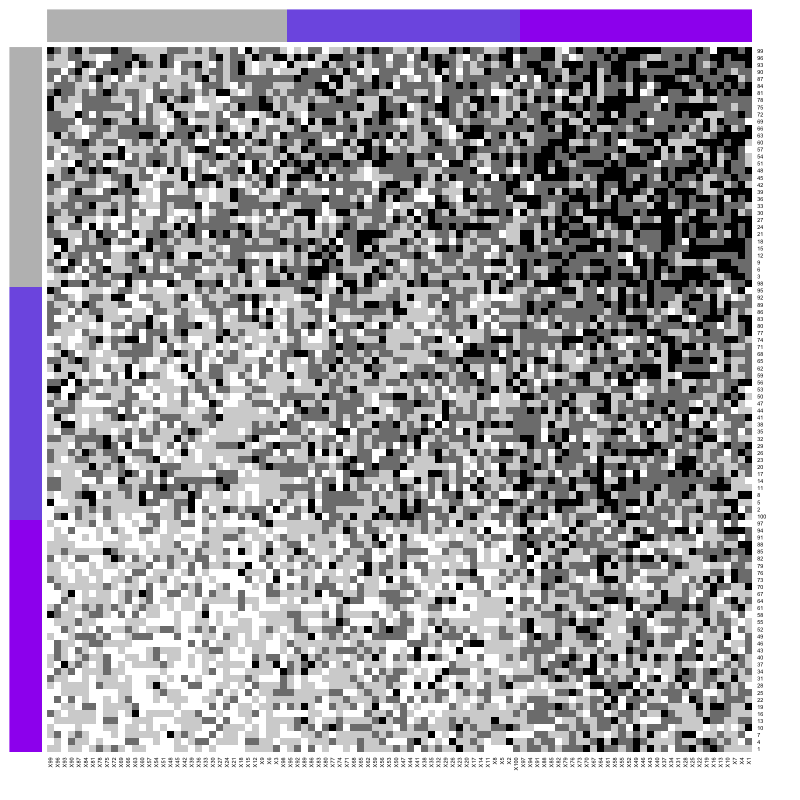
\includegraphics[width=.33\textwidth,natwidth=800,natheight=800]{ /Users/lapo_santi/Desktop/Nial/POMM_pairwise/POMMs/POMM_flex/MCMC/results_small_M/processed/adjacency_SimplePOMM_K3_N100.png}%
        \label{fig:simple_adjacency_K3}%
    }\hfill
    \subfigure[K=5, Simple Model]{%
        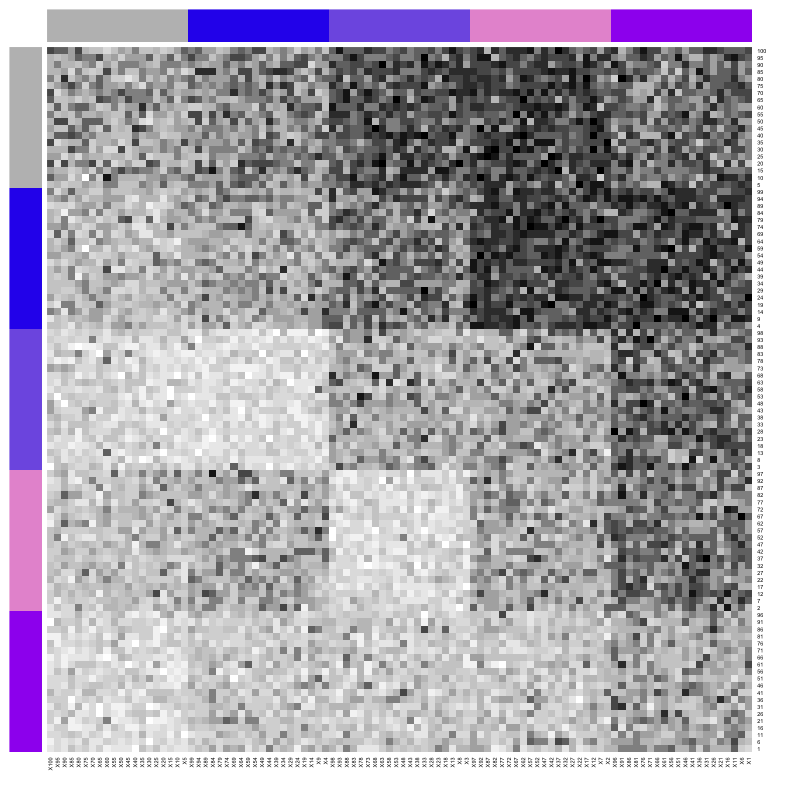
\includegraphics[width=.33\textwidth,natwidth=800,natheight=800]{ /Users/lapo_santi/Desktop/Nial/POMM_pairwise/POMMs/POMM_flex/MCMC/results_small_M/processed/adjacency_SimplePOMM_K5_N100.png}%
        \label{fig:simple_adjacency_K5}%
    }\hfill
    \subfigure[K=9, Simple Model]{%
        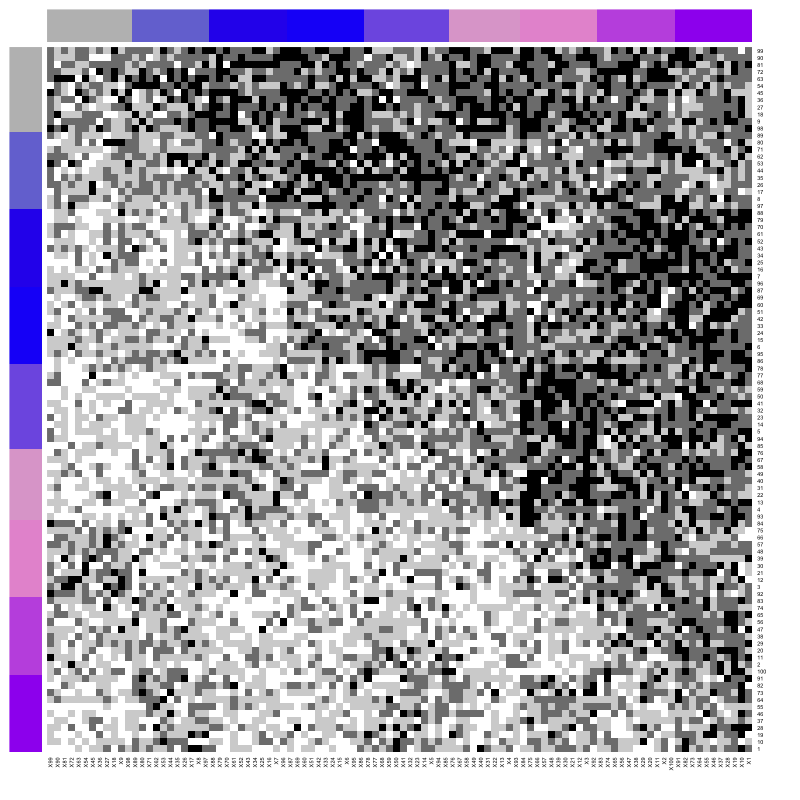
\includegraphics[width=.33\textwidth,natwidth=800,natheight=800]{ /Users/lapo_santi/Desktop/Nial/POMM_pairwise/POMMs/POMM_flex/MCMC/results_small_M/processed/adjacency_SimplePOMM_K9_N100.png}%
        \label{fig:simple_adjacency_K9}%
    }
    \caption{Adjacency Matrices simulated via the Simple Model}
    \label{fig:simple_adjacency}
\end{figure}

Each chain is initiated with different starting values and different seeds. The initiation values are saved in order to guarantee the reproducibility of the results.

For the POMM model, we need to choose an appropriate value for $\beta_{\max}$, which controls the maximum attainable value within the matrix $P$. Here we fix it arbitrarily at 0.85.



\begin{figure}[htbp]
    \centering
    \subfigure[K=3, Simple Model]{%
        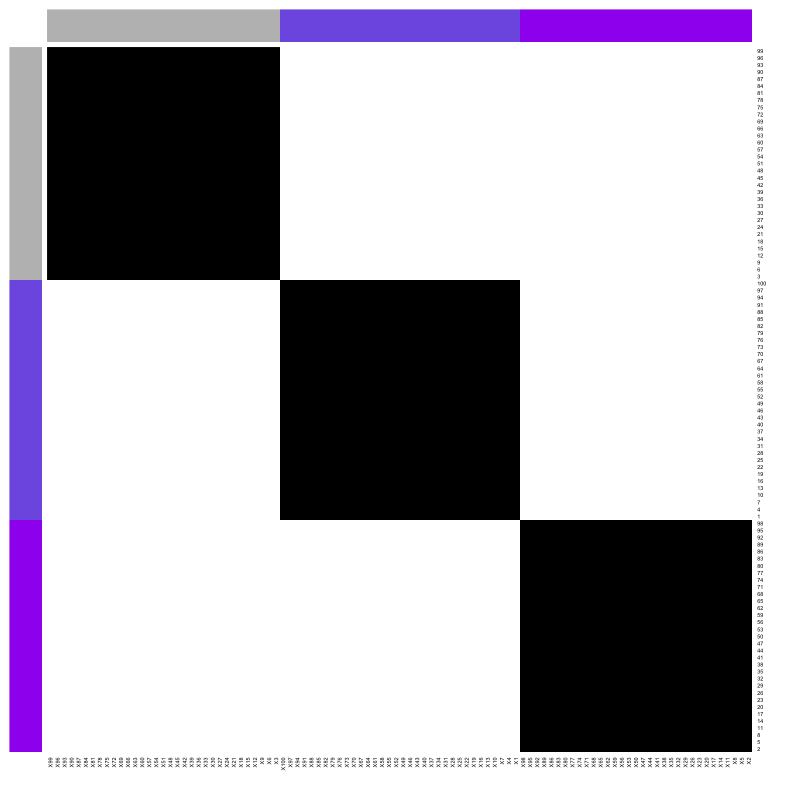
\includegraphics[width=.3333\textwidth,natwidth=800,natheight=800]{/Users/lapo_santi/Desktop/Nial/POMM_pairwise/POMMs/POMM_flex/MCMC/results_small_M/processed/similarity_SimpleSimpleK3_N100.png}%
        \label{fig:SimpleSimpleK3}%
    }\hfill
    \subfigure[K=5, Simple Model]{%
        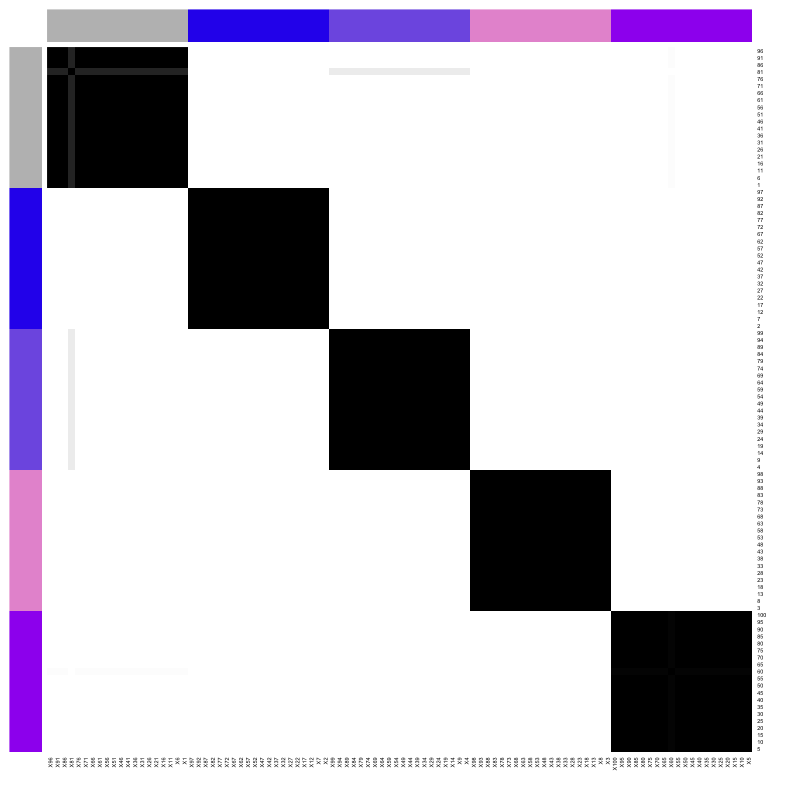
\includegraphics[width=.3333\textwidth,natwidth=800,natheight=800]{/Users/lapo_santi/Desktop/Nial/POMM_pairwise/POMMs/POMM_flex/MCMC/results_small_M/processed/similarity_SimpleSimpleK5_N100.png}%
        \label{fig:SimpleSimpleK5}%
    }\hfill
    \subfigure[K=9, Simple Model]{%
        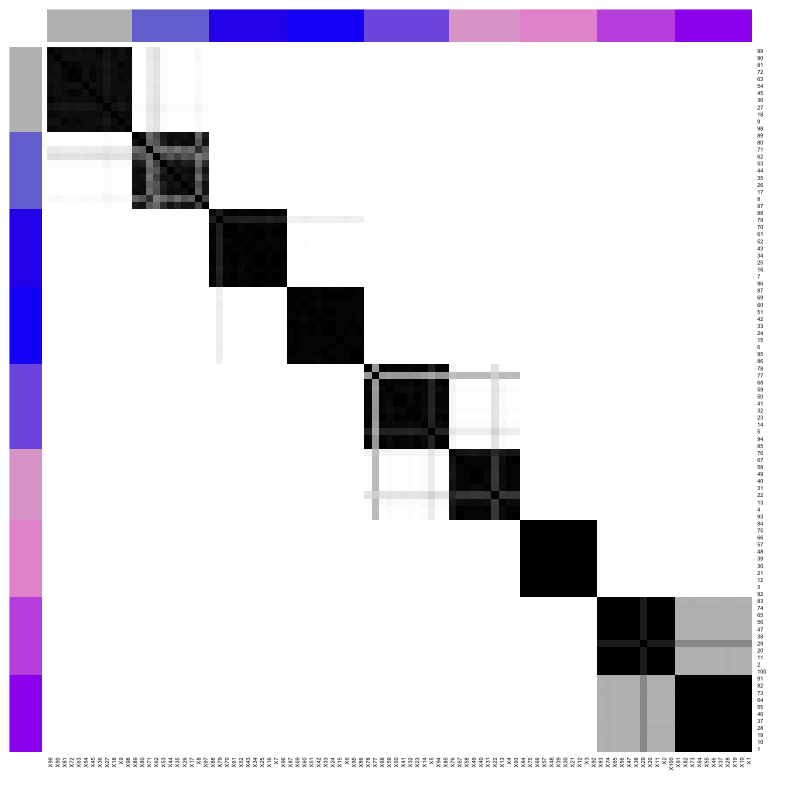
\includegraphics[width=.3333\textwidth,natwidth=800,natheight=800]{  /Users/lapo_santi/Desktop/Nial/POMM_pairwise/POMMs/POMM_flex/MCMC/results_29_07/tables_and_plots/plots/similarity_SimpleSimpleK9_N100.png}%
        \label{fig:SimpleSimpleK9}%
    }\\[2ex]\subfigure[K=3, POMM Model]{%
        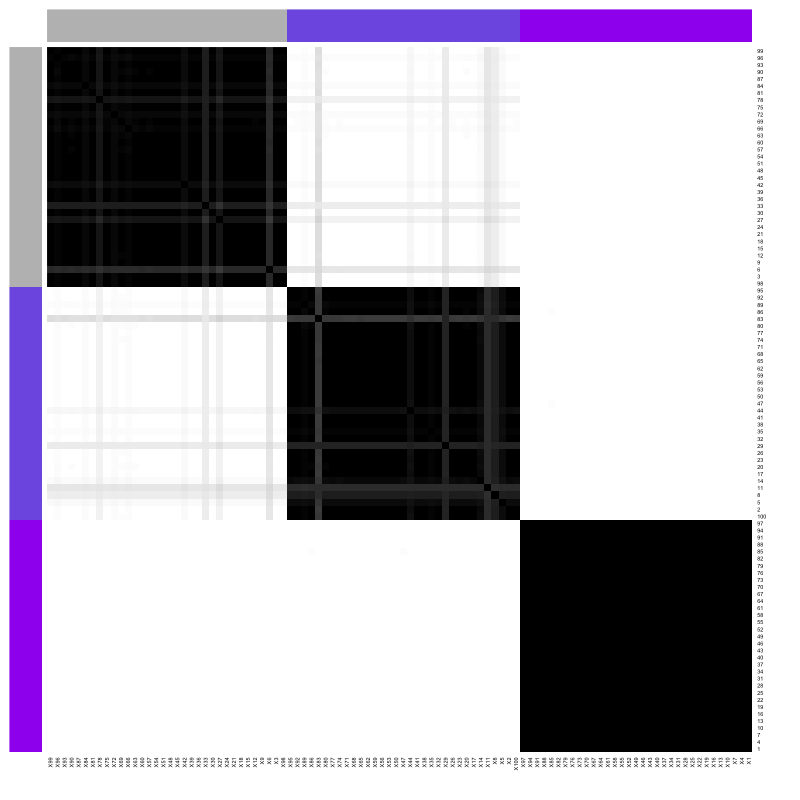
\includegraphics[width=.3333\textwidth,natwidth=800,natheight=800]{ /Users/lapo_santi/Desktop/Nial/POMM_pairwise/POMMs/POMM_flex/MCMC/results_small_M/processed/similarity_SimplePOMMK3_N100.png}%
        \label{fig:SimplePOMMK3}%
    }\hfill
    \subfigure[K=5, POMM Model]{%
        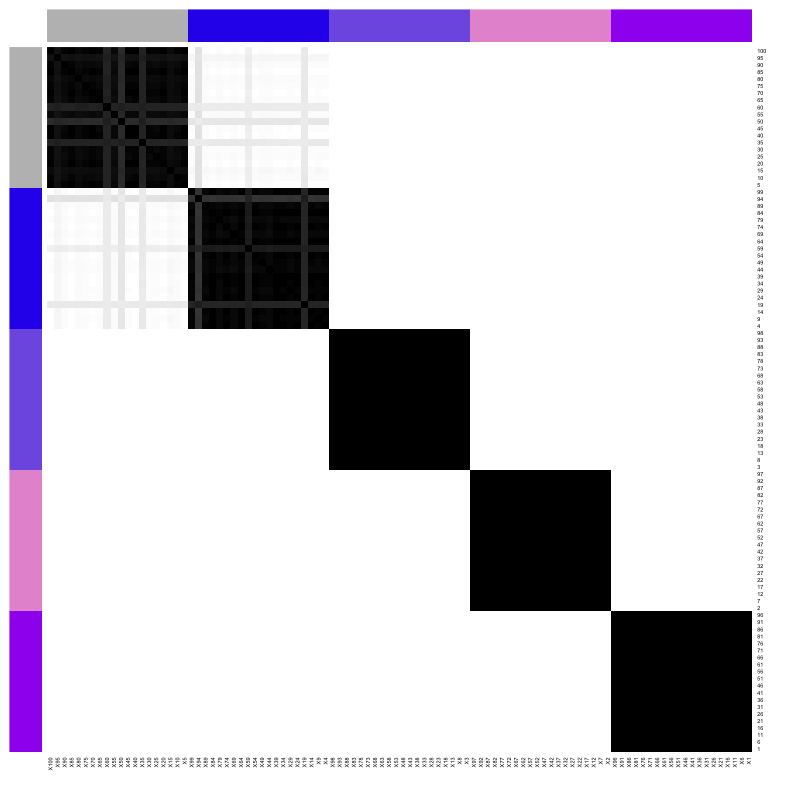
\includegraphics[width=.3333\textwidth,natwidth=800,natheight=800]{/Users/lapo_santi/Desktop/Nial/POMM_pairwise/POMMs/POMM_flex/MCMC/results_small_M/processed/similarity_SimplePOMMK5_N100.png}%
        \label{fig:SimplePOMMK5}%
    }\hfill
    \subfigure[K=9, POMM Model]{%
        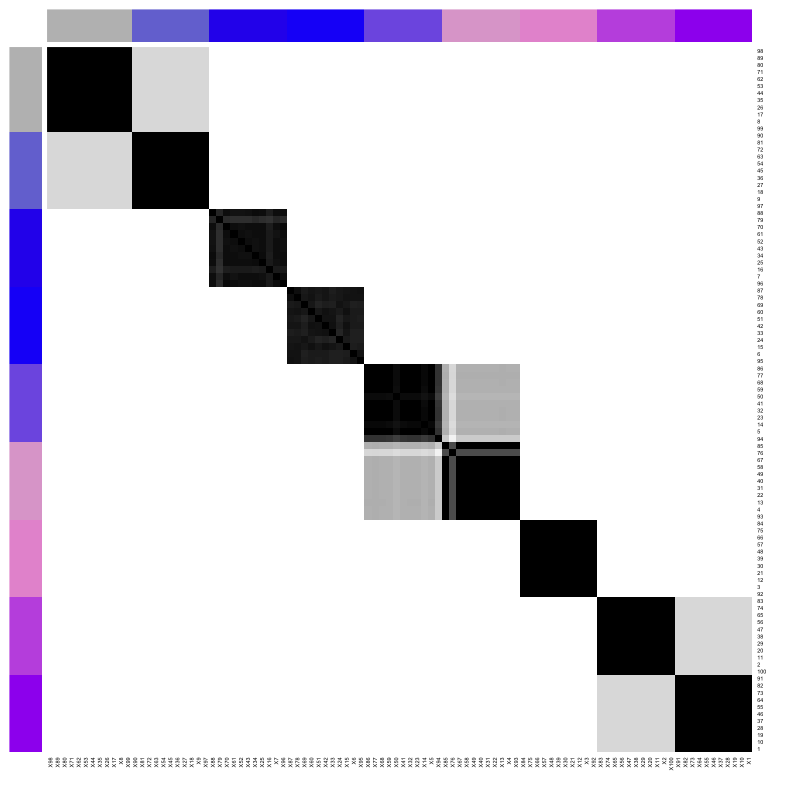
\includegraphics[width=.3333\textwidth,natwidth=800,natheight=800]{/Users/lapo_santi/Desktop/Nial/POMM_pairwise/POMMs/POMM_flex/MCMC/results_small_M/processed/similarity_SimplePOMMK9_N100.png}%
        \label{fig:SimplePOMMK9}%
    }
    \caption{Co-Clustering Matrices obtained via the Simple Model(above) and the POMM model (below).}
    \label{fig:similarity_all_simple}
\end{figure}

The first results' plot we report is the one in figure \eqref{fig:similarity_all_simple}. Each box contains a co-clustering matrix. Each pixel $(i,j)$ represents the probability that two individuals are placed within the same cluster. The darker the pixel, the higher the probability. Colours on the side signal the true membership of each player.

In the first row, containing figure \ref{fig:SimpleSimpleK3},figure \ref{fig:SimpleSimpleK5}, and figure \ref{fig:SimpleSimpleK9}, we have the co-clustering matrix for the Simple model estimated on the data generated according to the Simple model itself. This means that the blocks have no inherent ordering, and the model here is correctly specified. We can notice a very good recovery of the true membership.

In the second row instead, the one which contains figure \ref{fig:SimplePOMMK3},figure \ref{fig:SimplePOMMK5}, and \ref{fig:SimplePOMMK9}, we may observe the co-clustering matrix for the POMM model estimated on the data generated via the Simple one. Therefore, the model is misspecified, but we may notice that the recovery performance is quite competitive with the Simple one.



\begin{table}[htbp]
\centering
\caption{
{\large $P$ summary table} \\ 
{\small True Model Simple, $N=100$}
} 
\begin{tabular}{cccccccccc}
\toprule
\multirow{2}{*}{Fitted Model} & \multicolumn{3}{c}{
$MAE$ } & \multicolumn{3}{c}{
$\%$ within-95\% CI interval} & \multicolumn{3}{c}{ $\overline{\text{CI interval length}}$} \\
\cmidrule(lr){2-4} \cmidrule(lr){5-7} \cmidrule(lr){8-10}
& $(a)$ & $(b)$ & $(c)$ & $(a)$ & $(b)$ & $(c)$ & $(a)$ & $(b)$ & $(c)$ \\
\midrule
POMM model  &0.02 & 0.06 & 0.06 & 100 & 40 & 72.22 & 0.12 & 0.04 & 0.16 \\
Simple model & 0.00 & 0.06 & 0.06 & 100 & 50 & 69.44 & 0.02 & 0.10 & 0.15 \\
\bottomrule
\end{tabular}
\label{table:Psummary_simple}
\end{table}

In table \eqref{table:Psummary_simple}, we report the summary table of the estimates for the $P$ matrix, both obtained via the Simple model and the POMM model. For each value of $K$ (again, reported in the sub-columns (a), (b) and (c), respectively), we report the mean absolute error, meaning the mean absolute error $MAE = \frac{1}{(K\cdot(K-1))/2} \sum_{i=1}^{K-1}\sum_{j=i+1}^K \left(\hat{p}_{ij} - p^\star_{ij}\right)$ where $p^\star_{ij}$ is the true value of that particular entry. Then we also report the percentage of the upper triangular entries of $P$ that are contained by the estimated 95\% credible intervals, obtained by computing the 95\% higher posterior density region, and the average 95\% credible interval length. 

Here below, we report the ground truth of the $P$ matrix for each case $K=3,5,9$. Then, next and below we report the estimates, both for the POMM and the Simple model, within the $\hat{P}^{K=k}_{\text{POMM}}$, $\hat{P}^{K=k}_{\text{Simple}}$, respectively.

\newpage
\[
P^{K=3}_{true} = 
\left[\begin{array}{ccc}
0.500 & 0.586 & 0.736 \\
0.414 & 0.500 & 0.623 \\
0.264 & 0.377 & 0.500 \\
\end{array}\right] \quad 
\hat{P}^{K=3}_{\text{POMM}} = 
\left[\begin{array}{ccc}
0.500 & 0.600 & 0.754 \\
0.400 & 0.500 & 0.622 \\
0.246 & 0.378 & 0.500 \\
\end{array}\right] 
\]
\[ 
\hat{P}^{K=3}_{\text{Simple}} = 
\left[\begin{array}{ccc}
0.500 & 0.592 & 0.739 \\
0.408 & 0.500 & 0.627 \\
0.261 & 0.373 & 0.500 \\ 
\end{array}\right]
\]

\[
P^{K=5}_{true} = 
\left[\begin{array}{ccccc}
0.500 & 0.586 & 0.736 & 0.765 & 0.658 \\
0.414 & 0.500 & 0.623 & 0.782 & 0.768 \\
0.264 & 0.218 & 0.500 & 0.514 & 0.665 \\
0.377 & 0.486 & 0.232 & 0.500 & 0.637 \\
0.235 & 0.342 & 0.335 & 0.363 & 0.500 \\
\end{array}\right] \quad 
\hat{P}^{K=5}_{\text{POMM}} = 
\left[\begin{array}{ccccc}
0.500 & 0.589 & 0.731 & 0.687 & 0.718 \\
0.411 & 0.500 & 0.703 & 0.640 & 0.700 \\
0.269 & 0.297 & 0.500 & 0.643 & 0.658 \\
0.313 & 0.360 & 0.357 & 0.500 & 0.653 \\
0.282 & 0.300 & 0.342 & 0.347 & 0.500 \\
\end{array}\right] 
\]
\[ 
\hat{P}^{K=5}_{\text{Simple}} = 
\left[\begin{array}{ccccc}
0.500 & 0.566 & 0.660 & 0.700 & 0.710 \\
0.434 & 0.500 & 0.646 & 0.675 & 0.703 \\
0.340 & 0.354 & 0.500 & 0.666 & 0.665 \\
0.300 & 0.325 & 0.334 & 0.500 & 0.652 \\
0.290 & 0.297 & 0.335 & 0.348 & 0.500 \\
\end{array}\right]
\]

\[
P^{K=9}_{true} = 
\left[\begin{array}{ccccccccc}
0.500 & 0.586 & 0.736 & 0.765 & 0.658 & 0.787 & 0.770 & 0.708 & 0.587 \\
0.414 & 0.500 & 0.623 & 0.782 & 0.768 & 0.636 & 0.574 & 0.692 & 0.544 \\
0.264 & 0.335 & 0.500 & 0.514 & 0.665 & 0.703 & 0.513 & 0.798 & 0.789 \\
0.377 & 0.363 & 0.230 & 0.500 & 0.637 & 0.672 & 0.598 & 0.697 & 0.771 \\
0.235 & 0.213 & 0.426 & 0.292 & 0.500 & 0.531 & 0.786 & 0.713 & 0.707 \\
0.218 & 0.364 & 0.487 & 0.308 & 0.337 & 0.500 & 0.767 & 0.663 & 0.739 \\
0.486 & 0.297 & 0.402 & 0.202 & 0.322 & 0.211 & 0.500 & 0.678 & 0.507 \\
0.342 & 0.328 & 0.214 & 0.303 & 0.413 & 0.229 & 0.261 & 0.500 & 0.643 \\
0.232 & 0.469 & 0.233 & 0.287 & 0.456 & 0.293 & 0.493 & 0.357 & 0.500 \\\end{array}\right] 
\]
\[ 
\hat{P}^{K=9}_{\text{POMM}} = 
\left[\begin{array}{ccccccccc}
0.500 & 0.572 & 0.666 & 0.707 & 0.723 & 0.712 & 0.705 & 0.626 & 0.695 \\
0.428 & 0.500 & 0.646 & 0.689 & 0.716 & 0.725 & 0.667 & 0.656 & 0.635 \\
0.334 & 0.354 & 0.500 & 0.645 & 0.649 & 0.656 & 0.614 & 0.701 & 0.729 \\
0.293 & 0.311 & 0.355 & 0.500 & 0.651 & 0.666 & 0.666 & 0.687 & 0.751 \\
0.277 & 0.284 & 0.351 & 0.349 & 0.500 & 0.631 & 0.714 & 0.669 & 0.692 \\
0.288 & 0.275 & 0.344 & 0.334 & 0.369 & 0.500 & 0.667 & 0.732 & 0.674 \\
0.295 & 0.333 & 0.386 & 0.334 & 0.286 & 0.333 & 0.500 & 0.687 & 0.668 \\
0.374 & 0.344 & 0.299 & 0.313 & 0.331 & 0.268 & 0.313 & 0.500 & 0.603 \\
0.305 & 0.365 & 0.271 & 0.249 & 0.308 & 0.326 & 0.332 & 0.397 & 0.500 \\\end{array}\right] 
\]
\[ 
\hat{P}^{K=9}_{\text{Simple}} = 
\left[\begin{array}{ccccccccc}
0.500 & 0.601 & 0.675 & 0.711 & 0.702 & 0.744 & 0.702 & 0.659 & 0.709 \\
0.399 & 0.500 & 0.623 & 0.671 & 0.734 & 0.702 & 0.653 & 0.647 & 0.581 \\
0.325 & 0.377 & 0.500 & 0.652 & 0.640 & 0.653 & 0.624 & 0.691 & 0.720 \\
0.289 & 0.329 & 0.348 & 0.500 & 0.666 & 0.659 & 0.656 & 0.661 & 0.771 \\
0.298 & 0.266 & 0.360 & 0.334 & 0.500 & 0.631 & 0.709 & 0.671 & 0.686 \\
0.256 & 0.298 & 0.347 & 0.341 & 0.369 & 0.500 & 0.668 & 0.738 & 0.669 \\
0.298 & 0.347 & 0.376 & 0.344 & 0.291 & 0.332 & 0.500 & 0.734 & 0.617 \\
0.341 & 0.353 & 0.309 & 0.339 & 0.329 & 0.262 & 0.266 & 0.500 & 0.646 \\
0.291 & 0.419 & 0.280 & 0.229 & 0.314 & 0.331 & 0.383 & 0.354 & 0.500 \\\end{array}\right]
\]


\begin{table}[htbp]
\centering
\caption{
{\large $z$ summary table} \\ 
{\small True Model Simple, $N=100$}
} 
\begin{tabular}{cccccccccc}
\toprule
\multirow{2}{*}{Method} & \multicolumn{3}{c}{
VI $\text{distance}_{\text{MAP}}$} & \multicolumn{3}{c}{
VI $\text{distance}_{\text{VI lb}}$} & \multicolumn{3}{c}{WAIC} \\
\cmidrule(lr){2-4} \cmidrule(lr){5-7} \cmidrule(lr){8-10}
& $(a)$ & $(b)$ & $(c)$ & $(a)$ & $(b)$ & $(c)$ & $(a)$ & $(b)$ & $(c)$ \\
\midrule
POMM model  &0 & 0.42 & 0.1 & 0 & 0.42 & 0.32   & $\underset{30.89}{-13237.20}$ & $\underset{30.77}{-13352.68}$ & $\underset{31.35}{13657.35}$  \\
Simple model &0 & 0.42 & 0.1 & 0 & 0.42 & 0.32  & $\underset{31.16}{-13273.59}$ & $\underset{ 30.37}{-13293.26}$ & $\underset{31.34}{-13673.15}$ \\
\bottomrule
\end{tabular}
\label{table:z_summary_Simple}
\end{table}

In table \eqref{table:z_summary_Simple}, we report some summary statistics for the parameter $z$. As above, we have columns (a),(b) and (c) representing the case $K=3,5,9$ respectively.

The first indicator is the $VI \text{distance}_{\text{MAP}}$ computed between the true partition $z^\star$ and the point estimate $\hat{z}^{\text{MAP}}$ obtained with the maximum a posteriori estimate (MAP).

The second one is $VI \text{distance}_{\text{VI lb}}$ computed between the true partition $z^\star$ and the point estimate $\hat{z}^{\text{VI lb}}$ obtained with the partition attaining the VI lower bound.

The third one is the WAIC estimate, along with its standard error below.



\begin{table}[htbp]
\centering
\caption{
{\large POMM hyperparameters summary table} \\ 
{\small True Model Simple, $N=100$}
} 
\begin{tabular}{ccccccc}
\toprule
\multirow{2}{*}{Fitted Model} & \multicolumn{3}{c}{
$\hat{\theta}$} & \multicolumn{3}{c}{95$\%$ CI} \\
\cmidrule(lr){2-4} \cmidrule(lr){5-7} 
& $(a)$ & $(b)$ & $(c)$ & $(a)$ & $(b)$ & $(c)$  \\
\midrule
$\Sigma$  & 0.19 & 0.18 & 0.15 & [0.01	0.79] & [0.04	0.65] & [0.07	0.27]   \\
$\alpha$ & 0.60 & 0.41 & 0.23 & [0.24	0.9] & [0.11	0.75] & [0.1	0.4] \\
\bottomrule
\end{tabular}
\label{table:hyperparameters_SIMPLE}
\end{table}


In table \eqref{table:hyperparameters_SIMPLE}, we report the results for the hyperparameters of the $POMM$ model. In the $\hat{\theta}$ column we report the estimates both for $\alpha$ and $\Sigma$, while on the right we have their $95\%$ Credible Interval.
Given that the data were generated according the Simple model, we do not have a ground truth to which these results should be compared. However, we can still try to make sense of these values by inspecting the properties of the induced $P^{\text{POMM}}$ matrix resulting from the estimates.

The Simple model has a prior over $P^{\text{Simple}} \sim Beta(1,1)$, then we may expect $P^{\text{POMM}}$ itself to get as closer as needed to a uniform distribution by selecting the appropriate combination of $(\alpha, \Sigma)$. 

Therefore, we simulate $n=10000$ $P^{\text{POMM}}$ matrices via the estimated parameters $\hat{\theta}$ in \eqref{table:hyperparameters_SIMPLE}. Then we extract 1000 points from each level set to avoid sample biases, and we compare them with an equally-sized set simulated via the Simple model, using the Kolmogorov-Smirnov test, where the null hypothesis is that two sets of points are sampled from the same distribution.

\begin{table}[htbp]
\centering
\caption{
{\large Kolmogorov-Smirnov test} \\ 
{\small Data are generated via the estimated parameters}
} 
\begin{tabular}{ccccccc}
\toprule
\multirow{2}{*}{Method} & \multicolumn{3}{c}{
p-value} & \multicolumn{3}{c}{
$\%$ overlap between level sets} \\
\cmidrule(lr){2-4} \cmidrule(lr){5-7}
& $(a)$ & $(b)$ & $(c)$ & $(a)$ & $(b)$ & $(c)$  \\
\midrule
POMM model  &0.26& 0.05 & 0.00 & 82\% & 86\% & 89\% \\
\bottomrule
\end{tabular}
\label{table:ks_test}
\end{table}

In table \eqref{table:ks_test} we report first the Kolmogorov-Smirnov test p-values, and we may notice that for $K=3,5$ we do not reject with an $\alpha = 5\%$ that the $P^{\text{POMM}}$ is compatible with being extracted from the Simple model.

Instead with $K=9$ we cannot say that $P^{\text{POMM}}$ has collapsed to a uniform, but at the same time, if we look at the area of overlap between the densities of the level sets, we may notice that there is a significant amount of overlap between them, allowing the POMM model to effectively replicate the unordered entries of the $P^{\text{Simple}}$ matrix.


\begin{figure}[htbp]
    \centering
    \subfigure[K=3, $\alpha = 0.60, \Sigma =0.19$]{%
        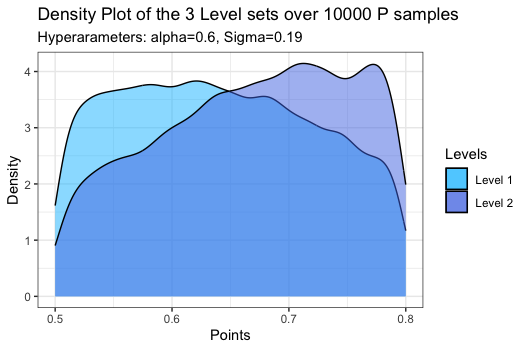
\includegraphics[width=.3333\textwidth,natwidth=528,natheight=350]{/Users/lapo_santi/Desktop/Nial/POMM_pairwise/POMMs/POMM_flex/MCMC/results_small_M/processed/LevelSets/Density_K3_simple.png}%
        \label{fig:Density_K3_simple}%
    }\hfill
    \subfigure[K=5, $\alpha = 0.41, \Sigma =0.18$]{%
        \includegraphics[width=.3333\textwidth,natwidth=528,natheight=350]{/Users/lapo_santi/Desktop/Nial/POMM_pairwise/POMMs/POMM_flex/MCMC/results_small_M/processed/LevelSets/Density_K5_simple.png}%
        \label{fig:Density_K5_simple}%
    }\hfill
    \subfigure[K=9, $\alpha = 0.23, \Sigma =0.15$]{%
        \includegraphics[width=.3333\textwidth,natwidth=528,natheight=350]{/Users/lapo_santi/Desktop/Nial/POMM_pairwise/POMMs/POMM_flex/MCMC/results_small_M/processed/LevelSets/Density_K9_simple.png}%
        \label{fig:Density_K9_simple}%
    }\\[2ex]\subfigure[K=3, $\alpha = 0.60, \Sigma =0.19$]{%
        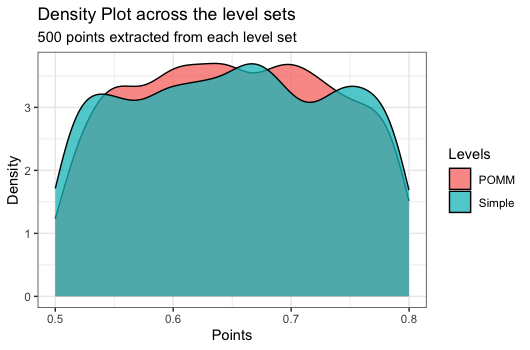
\includegraphics[width=.3333\textwidth,natwidth=528,natheight=350]{/Users/lapo_santi/Desktop/Nial/POMM_pairwise/POMMs/POMM_flex/MCMC/results_small_M/processed/LevelSets/Joint_K3.png}%
        \label{fig:Joint_K3}%
    }\hfill
    \subfigure[K=5, $\alpha = 0.41, \Sigma =0.18$]{%
        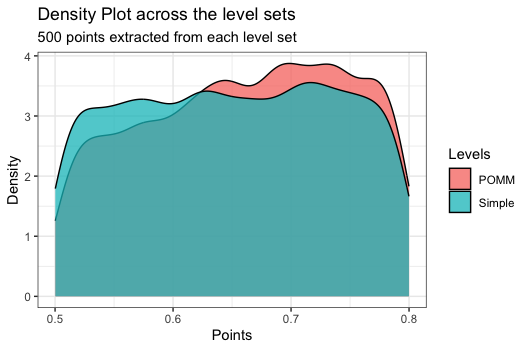
\includegraphics[width=.3333\textwidth,natwidth=528,natheight=350]{/Users/lapo_santi/Desktop/Nial/POMM_pairwise/POMMs/POMM_flex/MCMC/results_small_M/processed/LevelSets/Joint_K5.png}%
        \label{fig:Joint_K5}%
    }\hfill
    \subfigure[K=9, $\alpha = 0.23, \Sigma =0.15$]{%
        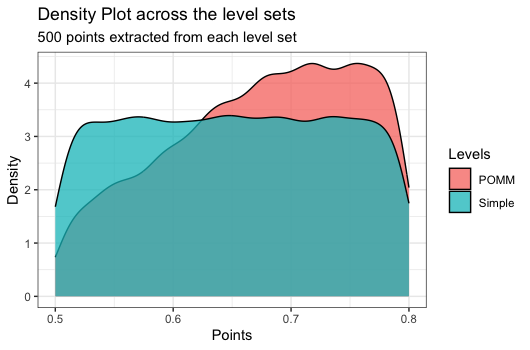
\includegraphics[width=.3333\textwidth,natwidth=528,natheight=350]{/Users/lapo_santi/Desktop/Nial/POMM_pairwise/POMMs/POMM_flex/MCMC/results_small_M/processed/LevelSets/Joint_K9.png}%
        \label{fig:Joint_K9}%
    }
    \caption{These are the densities of the entries of 10000 $P$ matrices generated according to the parameters within brackets, that is, the parameters estimated according the POMM model on the data generated via the Simple one. In figures  \eqref{fig:Density_K3_simple}, \eqref{fig:Density_K5_simple}, \eqref{fig:Density_K9_simple} we have the densities of the level sets coloured differently. In figures  \eqref{fig:Joint_K3}, \eqref{fig:Joint_K5}, \eqref{fig:Joint_K9} we put together 1000 points extracted from each level sets and we compute the density, so to have an overview of the joint distribution. We also compare the $P$'s entries simulated via the POMM and the Simple model}    
    \label{fig:overlapping_simple}
\end{figure}

In figure \eqref{fig:overlapping_simple} we report the densities of the points generated via the estimated hyper-parameters. We may notice the difference for the case $K=9$ with respect to the other two. In this case, we have very significant distributions for the POMM and the Simple one.


\clearpage




\subsubsection{Simple Model check}

In this subsection, we report some diagnostic checks for the algorithm of the Markov Chains, to assess convergence, quality of mixing, and the overall behaviour of the Metropolis-within-Gibbs algorithm.




\begin{table}[h]
\centering
\caption{
{\large $z$ diagnostic table} \\ 
{\small True Model Simple, $N=100$}
} 
\begin{tabular}{ccccccccccccc}
\toprule
\multirow{2}{*}{Fitted Model} & \multicolumn{3}{c}{$\overline{ESS}$} & \multicolumn{3}{c}{
$\overline{ACF_{30}}$} & \multicolumn{3}{c}{$\overline{\% accepted}$} & \multicolumn{3}{c}{$\overline{Gelman-Rubin}$}\\
\cmidrule(lr){2-4} \cmidrule(lr){5-7} \cmidrule(lr){8-10} \cmidrule(lr){11-13} 
& $(a)$ & $(b)$ & $(c)$ & $(a)$ & $(b)$ & $(c)$ & $(a)$ & $(b)$ & $(c)$ & $(a)$ & $(b)$ & $(c)$ \\
\midrule
POMM &7558.60 & 7988.02 & 2880.01 & 0 & 0.01 & 0.08 & 0.02 & 0.04 & 0.15 &  1.29 & 1.03 & 1.31  \\
Simple &6544.85 & 6688.51 & 2438.17 & 0 & 0.03 & 0.11 & 0.01 & 0.56 & 0.15 & 1.04 & 1.29 & 1.26   \\
\bottomrule
\end{tabular}
\label{table:z_diagnostics_simple}
\end{table}

In table \eqref{table:z_diagnostics_simple} we report the diagnostics for the $z$ parameter. Since the parameter is a label vector with 100 entries in this case, we compute the relevant statistics for each single entries an then we report the average.
\begin{itemize}

\item The first statistics is the Effective Sample Size (ESS) averaged over individuals $i=1,\dots,N$, which denotes a fairly good sample size. The average is taken as follows:

$$
\overline{ESS} = \frac{1}{n} \sum_{i=1}^N ESS_i
$$

The same is applied also to the other diagnostic metrics.

\item Then, we report the average autocorrelation, $\overline{ACF_{30}}$, computed with a lag of 30 iterations. This values are close to zero, meaning that there is very little correlation within the chain.

\item In the third column, we report the average acceptance rate $\overline{\% accepted}$. These are significantly lower than the target acceptance rate that should be hit by the adaptive MCMC, which is 22\%. However, the estimates are capable of correctly recovering the true partition. Combining the two facts, we may hypothesise that the simulation study has too "many" data, and proposing for a given individual $i$, who has already been assigned to the true block, a block different from the true one, leads to a drop in the likelihood which is too large, and as a consequence, we always reject the other labels. 

\item Finally, we compute the median Gelman-Rubin statistics for each entry, $\overline{Gelman-Rubin}$. Gelman and Rubin (1992) propose a general approach to monitoring convergence of MCMC output in which $m >1$ parallel chains are run with starting values that are overdispersed relative to the posterior distribution. Convergence is diagnosed when the chains have ‘forgotten’ their initial values, and the output from all chains is indistinguishable. The Gelman-Rubin diagnostic is applied to a single variable from the chain. It is based a comparison of within-chain and between-chain variances, and is similar to a classical analysis of variance. Values substantially above 1 indicate lack of convergence. If the chains have not converged,
\end{itemize}

\begin{table}[h]
\centering
\caption{
{\large $P$ diagnostic table} \\ 
{\small True Model Simple, $N=100$}
} 
\begin{tabular}{ccccccccccccc}
\toprule
\multirow{2}{*}{Fitted Model} & \multicolumn{3}{c}{$\overline{ESS}$} & \multicolumn{3}{c}{
$\overline{ACF_{30}}$} & \multicolumn{3}{c}{$\overline{\% accepted}$} & \multicolumn{3}{c}{$\overline{Gelman-Rubin}$}\\
\cmidrule(lr){2-4} \cmidrule(lr){5-7} \cmidrule(lr){8-10} \cmidrule(lr){11-13} 
& $(a)$ & $(b)$ & $(c)$ & $(a)$ & $(b)$ & $(c)$ & $(a)$ & $(b)$ & $(c)$ & $(a)$ & $(b)$ & $(c)$ \\
\midrule
POMM & 2234.00 & 2101.1 & 1454.08 & 0.02 & 0.00 & 0.15 & 34.52 & 31.55 & 29.98 & 1.06 & 1.0 & 1.04  \\
Simple &2742.67 & 1446.9 & 1565.14 & 0.00 & 0.13 & 0.17 & 36.85 & 31.01 & 30.06 & 1.00 & 1.9 & 1.03 \ \\
\bottomrule
\end{tabular}
\label{table:P_diagnostics_Simple}
\end{table}


In table \eqref{table:P_diagnostics_Simple} we report the same diagnostics checks for the $z$ parameter. The only difference is that here we do not average the diagnostics indicators over the individuals $i= 1,\ldots,N$, but instead over the upper-triangular $P$ indices: $\{ i =1,\ldots, K-1, \quad j = i+1, \ldots, K \}$.

Just as an example, the average ESS in this case is obtained as
$$
\overline{ESS} = \frac{1}{(K \cdot (K-1))/2} \sum_{i=1}^{N-1} \sum_{j=i+1}^N ESS_{i,j}
$$




\begin{table}[h]
\centering
\caption{
{\large POMM hyperparameters diagnostic table} \\ 
{\small True Model Simple, $N=100$}
} 
\begin{tabular}{ccccccccccccc}
\toprule
\multirow{2}{*}{Fitted Model} & \multicolumn{3}{c}{ESS} & \multicolumn{3}{c}{
ACF$_{30}$} & \multicolumn{3}{c}{$\%$ accepted} & \multicolumn{3}{c}{Gelman-Rubin}\\
\cmidrule(lr){2-4} \cmidrule(lr){5-7} \cmidrule(lr){8-10} \cmidrule(lr){11-13} 
& $(a)$ & $(b)$ & $(c)$ & $(a)$ & $(b)$ & $(c)$ & $(a)$ & $(b)$ & $(c)$ & $(a)$ & $(b)$ & $(c)$ \\
\midrule
$\Sigma$ &985 & 155 & 162 & 0.5 & 0.55 & 0.55 & 31.47 & 29.96 & 29.81 & 1.96 & 1.02 & 1.18 \\
$\alpha$ &13 & 17 & 45 & 0.95 & 0.94 & 0.84 & 24.74 & 24.93 & 24.38 & 1.21 & 1.62 & 1.01 \\
\bottomrule
\end{tabular}
\label{table:P_hyper_Simple}
\end{table}

Finally, in table \eqref{table:P_hyper_Simple} we report again the same diagnostics, but since both $\alpha$ and $\Sigma$ are one-dimensional, we are presenting the diagnostics itself, without any average.




\clearpage


\section{Simulation Study from the POMM Model N=100}

In this section we reverse the exercise performed in previous one. Before we were simulating from the Simple model, now we are doing the same, with similar parameters ($K=3,5,9, M=4000 \text{ and } \beta_{\max} = .75)$. Here are the results.

\begin{figure}[h]
    \centering
    \subfigure[K=3, POMM Model]{%
        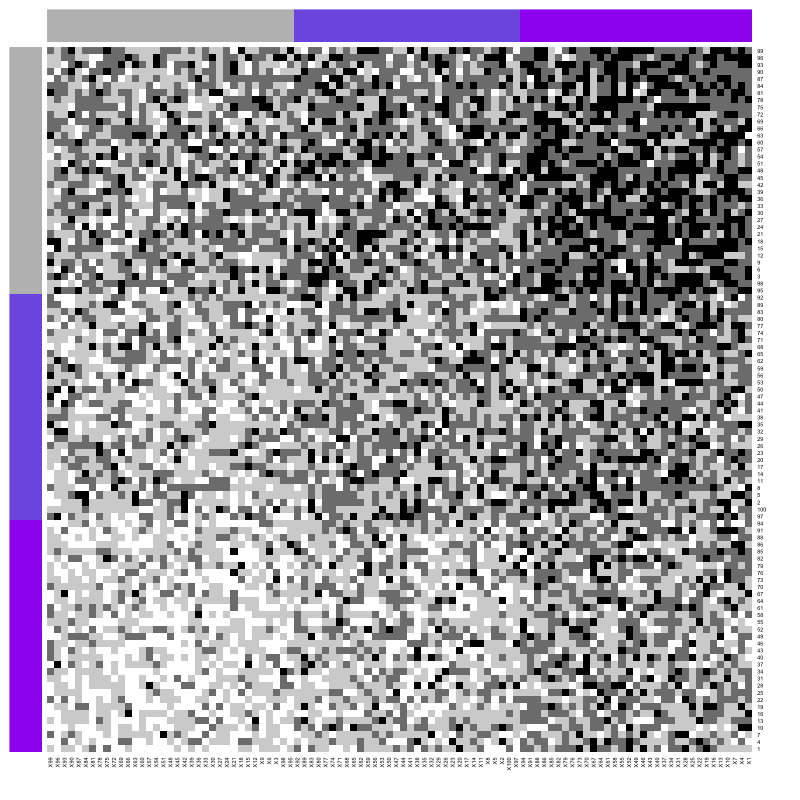
\includegraphics[width=.33\textwidth,natwidth=800,natheight=800]{/Users/lapo_santi/Desktop/Nial/POMM_pairwise/POMMs/POMM_flex/MCMC/results_small_M/processed/adjacency_POMMPOMM_K3_N100.png}%
        \label{fig:POMM_adjacency_K3}%
    }\hfill
    \subfigure[K=5, POMM Model]{%
        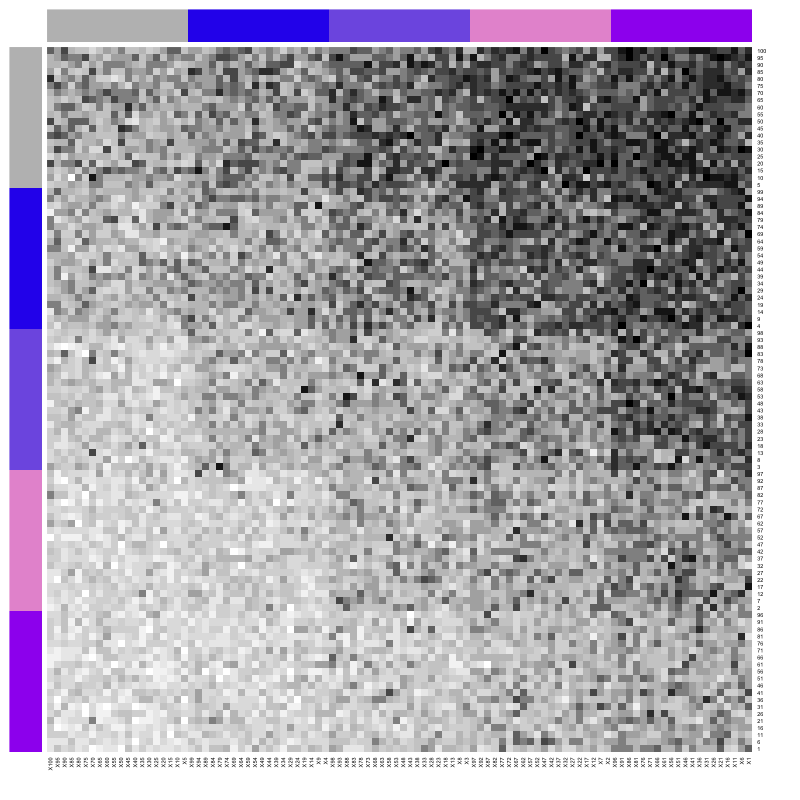
\includegraphics[width=.33\textwidth,natwidth=800,natheight=800]{/Users/lapo_santi/Desktop/Nial/POMM_pairwise/POMMs/POMM_flex/MCMC/results_small_M/processed/adjacency_POMMPOMM_K5_N100.png}%
        \label{fig:POMM_adjacency_K5}%
    }\hfill
    \subfigure[K=9, POMM Model]{%
        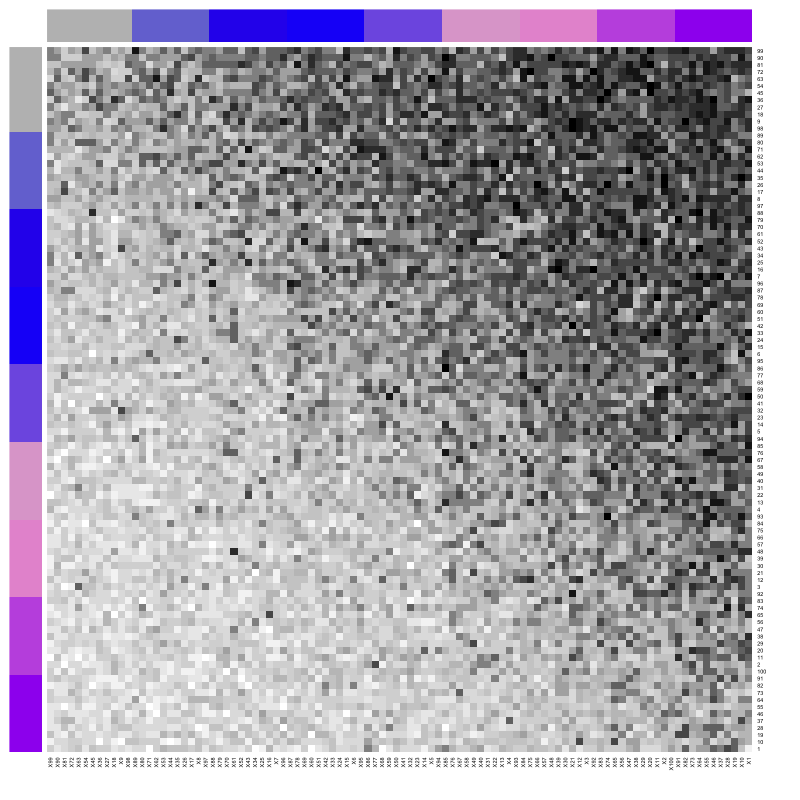
\includegraphics[width=.33\textwidth,natwidth=800,natheight=800]{/Users/lapo_santi/Desktop/Nial/POMM_pairwise/POMMs/POMM_flex/MCMC/results_small_M/processed/adjacency_POMMPOMM_K9_N100.png}%
        \label{fig:POMM_adjacency_K9}%
    }
    \caption{Adjacency Matrices simulated via the POMM Model}
    \label{fig:all_images}
\end{figure}

\begin{figure}[htbp]
    \centering
    \subfigure[K=3, Simple Model Estimates]{%
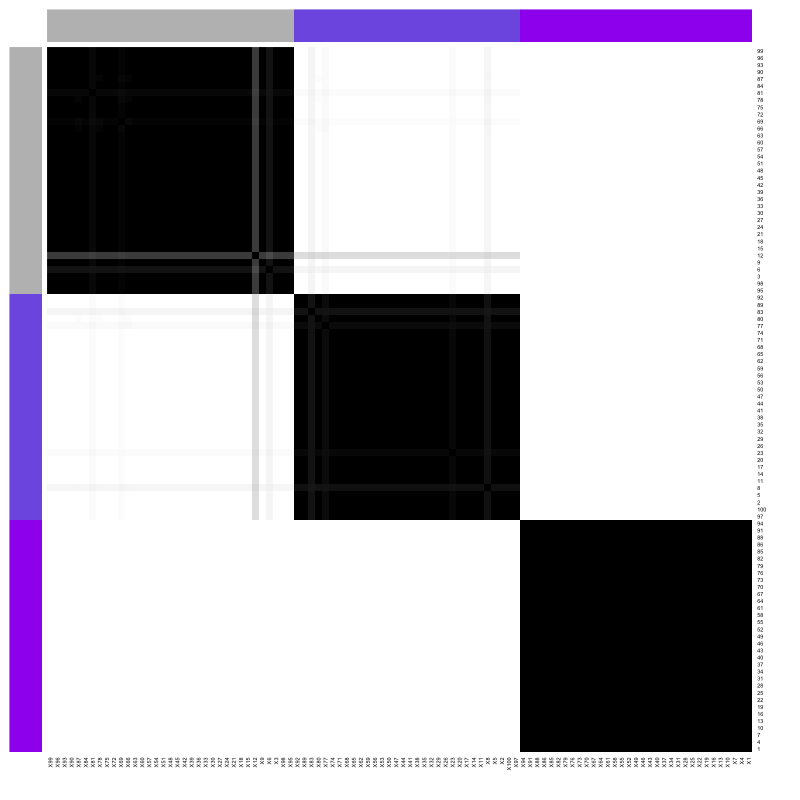
\includegraphics[width=.3333\textwidth,natwidth=800,natheight=800]{/Users/lapo_santi/Desktop/Nial/POMM_pairwise/POMMs/POMM_flex/MCMC/results_small_M/processed/similarity_POMMPOMMK3_N100.png}%
        \label{fig:M4000}%
    }\hfill
    \subfigure[K=5, Simple Model Estimates]{%
        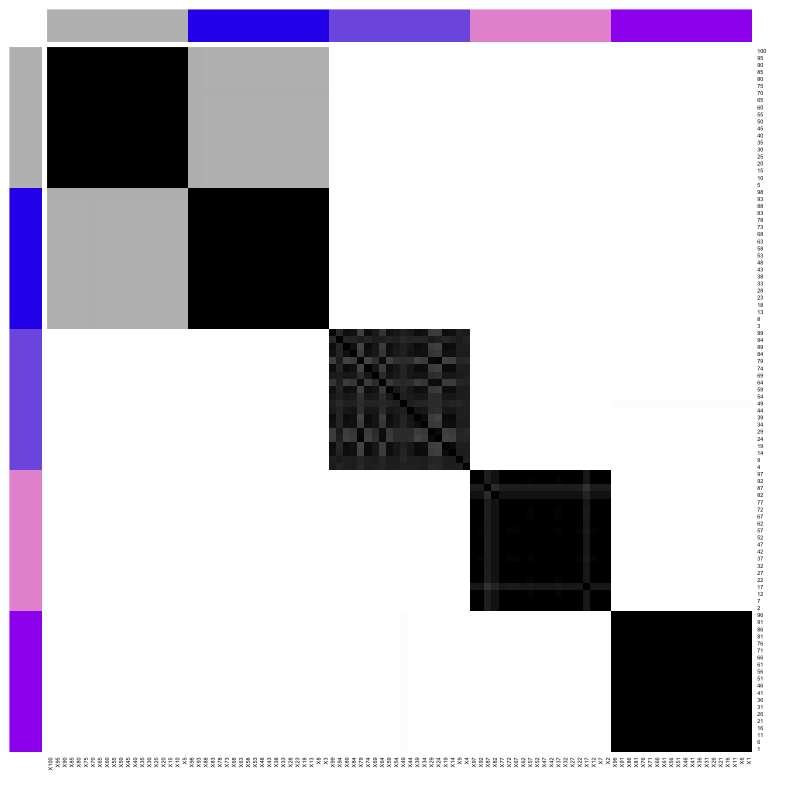
\includegraphics[width=.3333\textwidth,natwidth=800,natheight=800]{/Users/lapo_santi/Desktop/Nial/POMM_pairwise/POMMs/POMM_flex/MCMC/results_small_M/processed/similarity_POMMSimpleK5_N100.png}%
        \label{fig:M7000}%
    }\hfill
    \subfigure[K=9, Simple Model Estimates]{%
        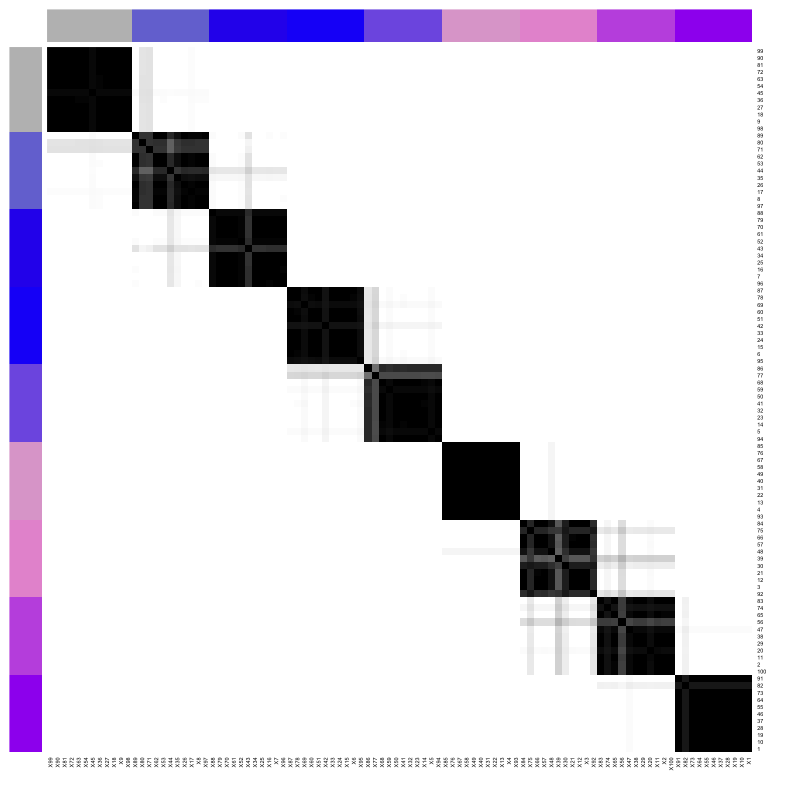
\includegraphics[width=.3333\textwidth,natwidth=800,natheight=800]{/Users/lapo_santi/Desktop/Nial/POMM_pairwise/POMMs/POMM_flex/MCMC/results_small_M/processed/similarity_POMMSimpleK9_N100.png}%
        \label{fig:M10000}%
    }\\[2ex]\subfigure[K=3, POMM Model Estimates]{%
        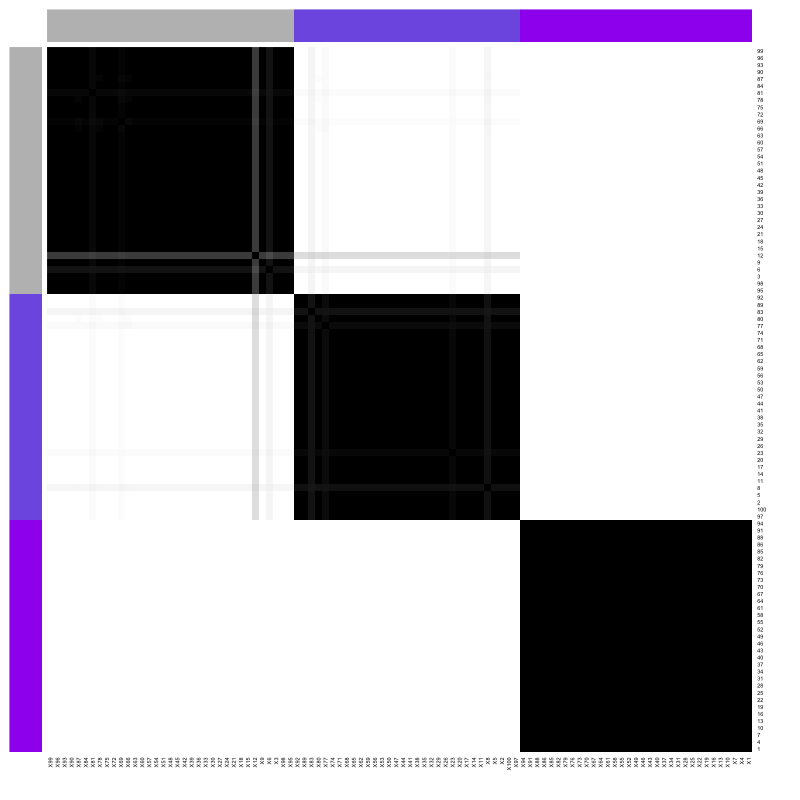
\includegraphics[width=.3333\textwidth,natwidth=800,natheight=800]{/Users/lapo_santi/Desktop/Nial/POMM_pairwise/POMMs/POMM_flex/MCMC/results_small_M/processed/similarity_POMMPOMMK3_N100.png}%
        \label{fig:M4000}%
    }\hfill
    \subfigure[K=5, POMM Model Estimates]{%
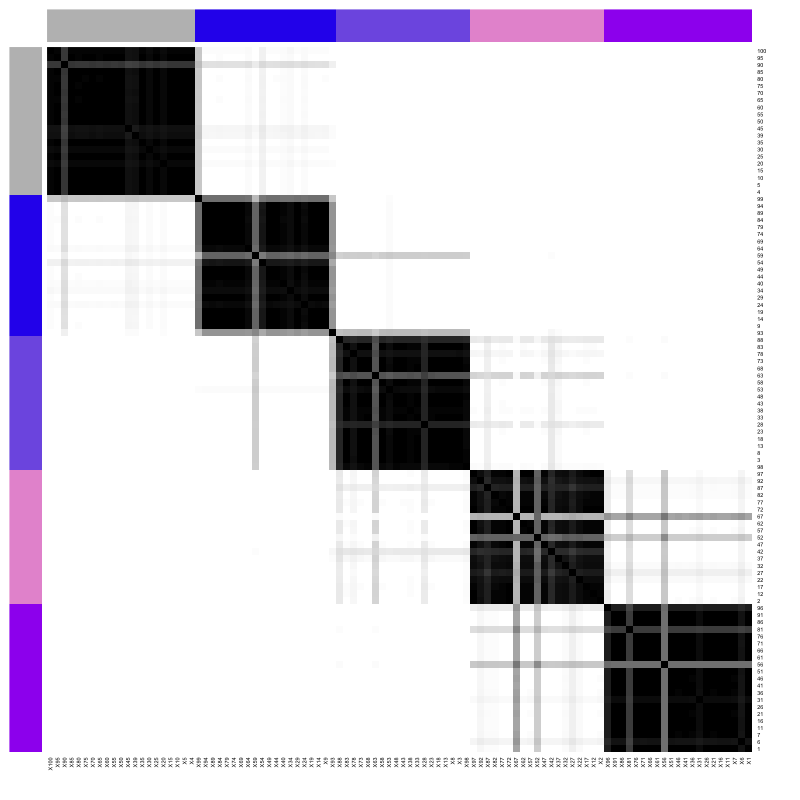
\includegraphics[width=.3333\textwidth,natwidth=800,natheight=800]{/Users/lapo_santi/Desktop/Nial/POMM_pairwise/POMMs/POMM_flex/MCMC/results_small_M/processed/similarity_POMMPOMMK5_N100.png}%
        \label{fig:M7000}%
    }\hfill
    \subfigure[K=9, POMM Model Estimates]{%
        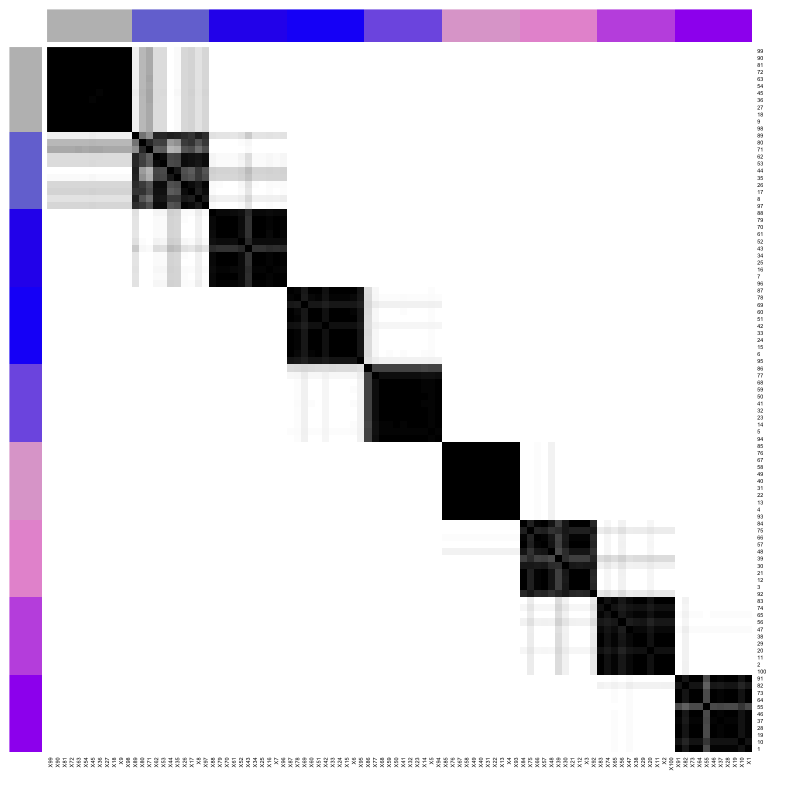
\includegraphics[width=.3333\textwidth,natwidth=800,natheight=800]{/Users/lapo_santi/Desktop/Nial/POMM_pairwise/POMMs/POMM_flex/MCMC/results_small_M/processed/similarity_POMMPOMMK9_N100.png}%
        \label{fig:M10000}%
    }
    \caption{Co-Clustering Matrices obtained via the Simple Model(above) and the POMM model (below).}
    \label{fig:all_images}
\end{figure}




\begin{table}[htbp]
\centering
\caption*{
{\large $P$ summary table} \\ 
{\small True Model POMM, $K=3$, $N=100$}
} 
\begin{tabular}{cccccccccc}
\toprule
\multirow{2}{*}{Fitted Model} & \multicolumn{3}{c}{
$\overline{MAE}$ } & \multicolumn{3}{c}{
$\%$ within-95\%-CI interval} & \multicolumn{3}{c}{ $\overline{\text{CI interval length}}$} \\
\cmidrule(lr){2-4} \cmidrule(lr){5-7} \cmidrule(lr){8-10}
& $(a)$ & $(b)$ & $(c)$ & $(a)$ & $(b)$ & $(c)$ & $(a)$ & $(b)$ & $(c)$ \\
\midrule
POMM model  &0.02 & 0.02 & 0.01 & 100\% & 90\% & 61.11\% & 0.14 & 0.08 & 0.02  \\
Simple model & 0.00 & 0.04 & 0.02 & 100\% & 90\% & 100.00\% & 0.02 & 0.11 & 0.15 \\
\bottomrule
\end{tabular}
\label{table:simulations_from_simple}
\end{table}

\newpage
\[
P^{K=3}_{true} = 
\left[\begin{array}{ccc}
0.500 & 0.600 & 0.754 \\
0.400 & 0.500 & 0.622 \\
0.246 & 0.378 & 0.500 \\ 
\end{array}\right] \quad 
\hat{P}^{K=3}_{\text{POMM}} = 
\left[\begin{array}{ccc}
0.500 & 0.582 & 0.726 \\
0.418 & 0.500 & 0.649 \\
0.274 & 0.351 & 0.500 \\ 
\end{array}\right] 
\]
\[ 
\hat{P}^{K=3}_{\text{Simple}} = 
\left[\begin{array}{ccc}
0.500 & 0.606 & 0.758 \\
0.394 & 0.500 & 0.623 \\
0.242 & 0.377 & 0.500 \\ 
\end{array}\right]
\]

\[
P^{K=5}_{true} = 
\left[\begin{array}{ccccc}
0.500 & 0.569 & 0.679 & 0.752 & 0.781 \\
0.431 & 0.500 & 0.576 & 0.698 & 0.741 \\
0.321 & 0.424 & 0.500 & 0.562 & 0.674 \\
0.248 & 0.302 & 0.438 & 0.500 & 0.571 \\
0.219 & 0.259 & 0.326 & 0.429 & 0.500 \\
\end{array}\right] \quad   
\hat{P}^{K=5}_{\text{POMM}} = 
\left[\begin{array}{ccccc}
0.500 & 0.575 & 0.694 & 0.723 & 0.775 \\
0.425 & 0.500 & 0.604 & 0.655 & 0.736 \\
0.306 & 0.396 & 0.500 & 0.555 & 0.655 \\
0.277 & 0.345 & 0.445 & 0.500 & 0.597 \\
0.225 & 0.264 & 0.345 & 0.403 & 0.500 \\
\end{array}\right] 
\]
\[ 
\hat{P}^{K=5}_{\text{Simple}} = 
\left[\begin{array}{ccccc}
0.500 & 0.557 & 0.681 & 0.703 & 0.761 \\
0.443 & 0.500 & 0.659 & 0.641 & 0.744 \\
0.319 & 0.341 & 0.500 & 0.532 & 0.625 \\
0.297 & 0.359 & 0.468 & 0.500 & 0.622 \\
0.239 & 0.256 & 0.375 & 0.378 & 0.500 \\
\end{array}\right]
\]

\[
P^{K=9}_{true} = 
\left[\begin{array}{ccccccccc}
0.500 & 0.547 & 0.626 & 0.682 & 0.699 & 0.726 & 0.766 & 0.775 & 0.778 \\
0.453 & 0.500 & 0.546 & 0.624 & 0.679 & 0.702 & 0.729 & 0.750 & 0.765 \\
0.374 & 0.454 & 0.500 & 0.571 & 0.633 & 0.647 & 0.705 & 0.720 & 0.738 \\
0.318 & 0.376 & 0.429 & 0.500 & 0.551 & 0.618 & 0.660 & 0.692 & 0.708 \\
0.301 & 0.321 & 0.367 & 0.449 & 0.500 & 0.561 & 0.630 & 0.655 & 0.710 \\
0.274 & 0.298 & 0.353 & 0.382 & 0.439 & 0.500 & 0.557 & 0.625 & 0.676 \\
0.234 & 0.271 & 0.295 & 0.340 & 0.370 & 0.443 & 0.500 & 0.562 & 0.636 \\
0.225 & 0.250 & 0.280 & 0.308 & 0.345 & 0.375 & 0.438 & 0.500 & 0.560 \\
0.222 & 0.235 & 0.262 & 0.292 & 0.290 & 0.324 & 0.364 & 0.440 & 0.500 \\
\end{array}\right] 
\]
\[ 
\hat{P}^{K=9}_{\text{POMM}} = 
\left[\begin{array}{ccccccccc}
0.500 & 0.559 & 0.637 & 0.674 & 0.704 & 0.729 & 0.754 & 0.773 & 0.791 \\
0.441 & 0.500 & 0.558 & 0.637 & 0.675 & 0.704 & 0.730 & 0.751 & 0.772 \\
0.363 & 0.442 & 0.500 & 0.559 & 0.637 & 0.674 & 0.704 & 0.730 & 0.752 \\
0.326 & 0.363 & 0.441 & 0.500 & 0.557 & 0.636 & 0.675 & 0.704 & 0.729 \\
0.296 & 0.325 & 0.363 & 0.443 & 0.500 & 0.557 & 0.638 & 0.676 & 0.705 \\
0.271 & 0.296 & 0.326 & 0.364 & 0.443 & 0.500 & 0.557 & 0.637 & 0.675 \\
0.246 & 0.270 & 0.296 & 0.325 & 0.362 & 0.443 & 0.500 & 0.558 & 0.638 \\
0.227 & 0.249 & 0.270 & 0.296 & 0.324 & 0.363 & 0.442 & 0.500 & 0.558 \\
0.209 & 0.228 & 0.248 & 0.271 & 0.295 & 0.325 & 0.362 & 0.442 & 0.500 \\
\end{array}\right] 
\]
\[ 
\hat{P}^{K=9}_{\text{Simple}} = 
\left[\begin{array}{ccccccccc}
0.500 & 0.547 & 0.626 & 0.682 & 0.699 & 0.726 & 0.766 & 0.775 & 0.778 \\
0.453 & 0.500 & 0.546 & 0.624 & 0.679 & 0.702 & 0.729 & 0.750 & 0.765 \\
0.374 & 0.454 & 0.500 & 0.571 & 0.633 & 0.647 & 0.705 & 0.720 & 0.738 \\
0.318 & 0.376 & 0.429 & 0.500 & 0.551 & 0.618 & 0.660 & 0.692 & 0.708 \\
0.301 & 0.321 & 0.367 & 0.449 & 0.500 & 0.561 & 0.630 & 0.655 & 0.710 \\
0.274 & 0.298 & 0.353 & 0.382 & 0.439 & 0.500 & 0.557 & 0.625 & 0.676 \\
0.234 & 0.271 & 0.295 & 0.340 & 0.370 & 0.443 & 0.500 & 0.562 & 0.636 \\
0.225 & 0.250 & 0.280 & 0.308 & 0.345 & 0.375 & 0.438 & 0.500 & 0.560 \\
0.222 & 0.235 & 0.262 & 0.292 & 0.290 & 0.324 & 0.364 & 0.440 & 0.500 \\ \\\end{array}\right]
\]



\begin{table}[htbp]
\centering
\caption*{
{\large $z$ summary table} \\ 
{\small True Model POMM, $N=100$}
} 
\begin{tabular}{cccccccccc}
\toprule
\multirow{2}{*}{Method} & \multicolumn{3}{c}{
VI $\text{distance}_{\text{MAP}}$} & \multicolumn{3}{c}{
VI $\text{distance}_{\text{VI lb}}$} & \multicolumn{3}{c}{WAIC} \\
\cmidrule(lr){2-4} \cmidrule(lr){5-7} \cmidrule(lr){8-10}
& $(a)$ & $(b)$ & $(c)$ & $(a)$ & $(b)$ & $(c)$ & $(a)$ & $(b)$ & $(c)$ \\
\midrule
POMM model  &0.13 & 0.53 & 1.9 & 0.13 & 0.42 & 1.73  & $\underset{30.98}{-13361.79}$ & $\underset{31.45}{-13510.00}$ & $\underset{31.03}{-13645.28}$  \\
Simple model & 0.13 & 0.31 & 2.0 & 0.13 & 0.48 & 1.71 & $\underset{30.74}{-13409.44}$ & $\underset{31.71}{-13496.19}$ & $\underset{30.71}{-13659.10}$ \\
\bottomrule
\end{tabular}
\label{table:z_summary_POMM}
\end{table}


\begin{table}[htbp]
\centering
\caption{
{\large POMM Hyperparameters summary table} \\ 
{\small True Model POMM, $N=100$}
} 
\begin{tabular}{cccccccccc}
\toprule
\multirow{2}{*}{Method} & \multicolumn{3}{c}{
$\hat{\theta}$} & \multicolumn{3}{c}{
95$\%$ CI interval} & \multicolumn{3}{c}{True value} \\
\cmidrule(lr){2-4} \cmidrule(lr){5-7} \cmidrule(lr){8-10}
& $(a)$ & $(b)$ & $(c)$ & $(a)$ & $(b)$ & $(c)$ & $(a)$ & $(b)$ & $(c)$ \\
\midrule
$\Sigma$ &0.1487 & 0.084 & 0.0196 & [0.0033	0.7575] & [4e-04	0.5602] & [0.0012	0.0625] & 0.01 & 0.01 & 0.01   \\
$\alpha$ & 0.4237 & 0.5265 & 0.491 & [0.1324	0.6215] & [0.439	0.8733] & [0.4258	0.5934] & 0.5 & 0.5 & 0.5 \\
\bottomrule
\end{tabular}
\label{table:hyper_summary_POMM}
\end{table}


\subsection{POMM model check}



\begin{table}[htbp]
\centering
\caption*{
{\large $z$ diagnostic table} \\ 
{\small True Model POMM, $N=100$}
} 
\begin{tabular}{ccccccccccccc}
\toprule
\multirow{2}{*}{Fitted Model} & \multicolumn{3}{c}{ESS} & \multicolumn{3}{c}{
ACF$_{30}$} & \multicolumn{3}{c}{$\%$ accepted} & \multicolumn{3}{c}{Gelman-Rubin}\\
\cmidrule(lr){2-4} \cmidrule(lr){5-7} \cmidrule(lr){8-10} \cmidrule(lr){11-13} 
& $(a)$ & $(b)$ & $(c)$ & $(a)$ & $(b)$ & $(c)$ & $(a)$ & $(b)$ & $(c)$ & $(a)$ & $(b)$ & $(c)$ \\
\midrule
POMM &3418.94 & 10354.90 & 4800.38 & 0.11 & 0.02 & 0.09 & 0.01 & 0.33 & 4.50 &  1.29 & 1.08 & 1.00    \\
Simple &1778.56 & 10191.58 & 1869.04 & 0.00 & 0.01 & 0.36 & 0.01 & 0.50 & 2.64 & 1.02 & 1.17 & 1.08 \\
\bottomrule
\end{tabular}
\label{table:z_diagnostic_POMM}
\end{table}

\begin{table}[htbp]
\centering
\caption*{
{\large $P$ diagnostic table} \\ 
{\small True Model POMM, $N=100$}
} 
\begin{tabular}{ccccccccccccc}
\toprule
\multirow{2}{*}{Fitted Model} & \multicolumn{3}{c}{ESS} & \multicolumn{3}{c}{
ACF$_{30}$} & \multicolumn{3}{c}{$\%$ accepted} & \multicolumn{3}{c}{Gelman-Rubin}\\
\cmidrule(lr){2-4} \cmidrule(lr){5-7} \cmidrule(lr){8-10} \cmidrule(lr){11-13} 
& $(a)$ & $(b)$ & $(c)$ & $(a)$ & $(b)$ & $(c)$ & $(a)$ & $(b)$ & $(c)$ & $(a)$ & $(b)$ & $(c)$ \\
\midrule
POMM &626.67 & 672.7 & 308.22 & 0.29 & 0.22 & 0.34 & 20.89 & 29.75 & 29.55 & 1.36 & 1.34 & 1.11    \\
Simple &2798.00 & 1659.7 & 121.94 & 0.00 & 0.02 & 0.53 & 36.70 & 30.99 & 29.78 & 1.00 & 1.07 & 1.03    \\
\bottomrule
\end{tabular}
\label{table:P_diagnostic_POMM}
\end{table}




\begin{table}[htbp]
\centering
\caption*{
{\large POMM hyperparameters diagnostic table} \\ 
{\small True Model POMM, $N=100$}
} 
\begin{tabular}{ccccccccccccc}
\toprule
\multirow{2}{*}{Fitted Model} & \multicolumn{3}{c}{ESS} & \multicolumn{3}{c}{
ACF$_{30}$} & \multicolumn{3}{c}{$\%$ accepted} & \multicolumn{3}{c}{Gelman-Rubin}\\
\cmidrule(lr){2-4} \cmidrule(lr){5-7} \cmidrule(lr){8-10} \cmidrule(lr){11-13} 
& $(a)$ & $(b)$ & $(c)$ & $(a)$ & $(b)$ & $(c)$ & $(a)$ & $(b)$ & $(c)$ & $(a)$ & $(b)$ & $(c)$ \\
\midrule
$\Sigma$ &981 & 480 & 13 & 0.4 & 0.58 & 0.94 & 15.78 & 11.38 & 1.72 & 3.55 & 2.15 & 1.96  \\
$\alpha$ &59 & 85 & 29 & 0.8 & 0.71 & 0.88 & 16.32 & 15.41 & 6.33 & 1.26 & 1.35 & 1.25    \\
\bottomrule
\end{tabular}
\label{table:simulations_from_simple}
\end{table}






\clearpage

\section{Application to Tennis Data}


\begin{figure}[h]
    \centering
    \subfigure[K=3, Simple Model]{%
        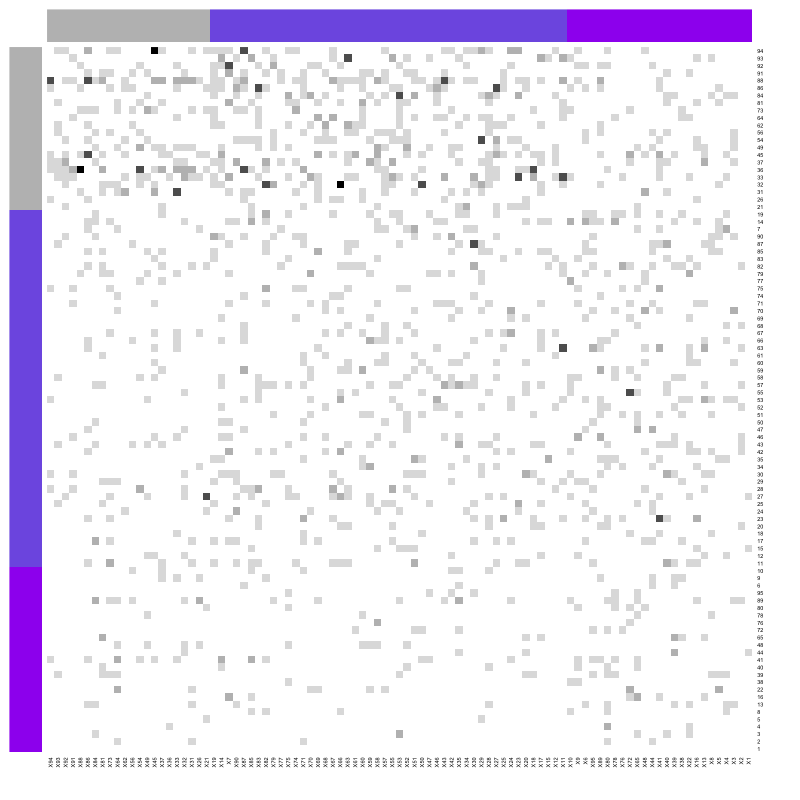
\includegraphics[width=.33\textwidth,natwidth=800,natheight=800]{/Users/lapo_santi/Desktop/Nial/POMM_pairwise/POMMs/Tennis application/results/processed_results/adjacency_Tennis_application_Est_model_Simple_K3_N95.png}%
        \label{fig:POMM_adjacency_K3}%
    }\hfill
    \subfigure[K=4, Simple Model]{%
        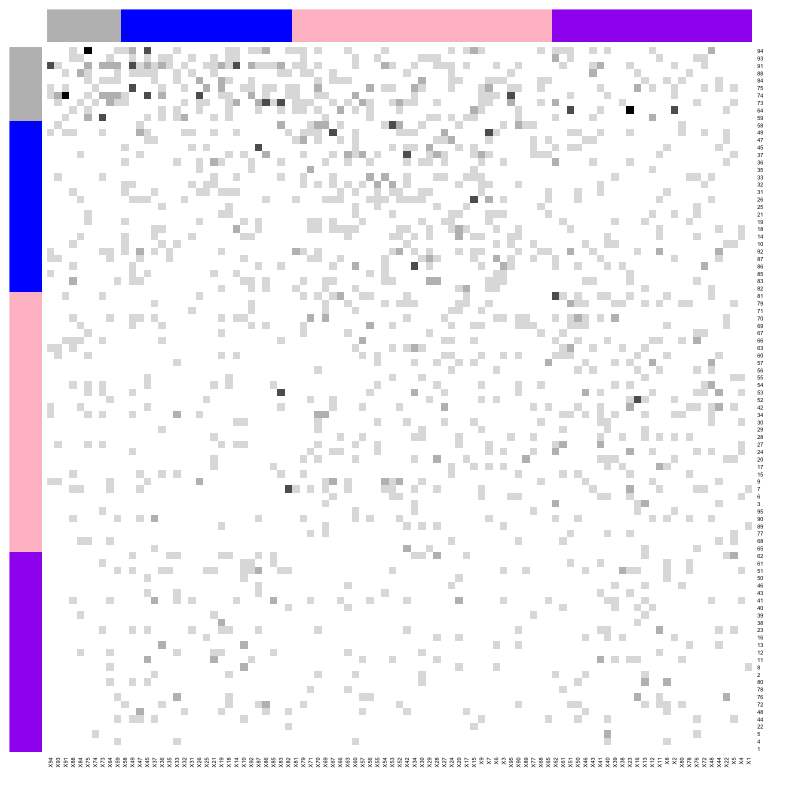
\includegraphics[width=.33\textwidth,natwidth=800,natheight=800]{/Users/lapo_santi/Desktop/Nial/POMM_pairwise/POMMs/Tennis application/results/processed_results/adjacency_Tennis_application_Est_model_Simple_K4_N95.png}%
        \label{fig:POMM_adjacency_K5}%
    }\hfill
    \subfigure[K=5, Simple Model]{%
        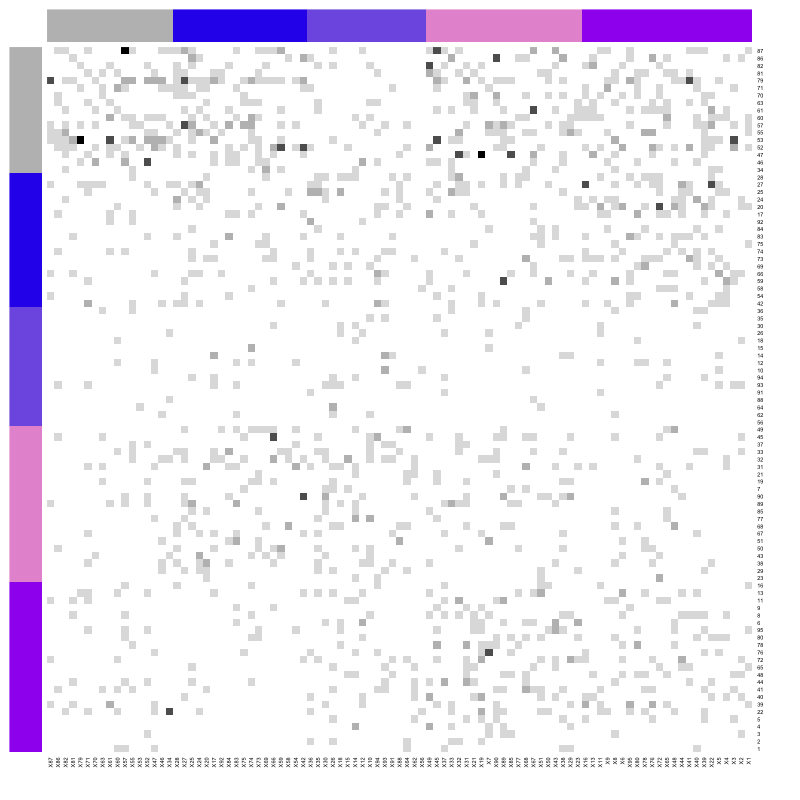
\includegraphics[width=.33\textwidth,natwidth=800,natheight=800]{/Users/lapo_santi/Desktop/Nial/POMM_pairwise/POMMs/Tennis application/results/processed_results/adjacency_Tennis_application_Est_model_Simple_K5_N95.png}%
        \label{fig:POMM_adjacency_K9}%
    }\\[2ex]\subfigure[K=3, POMM Model]{%
        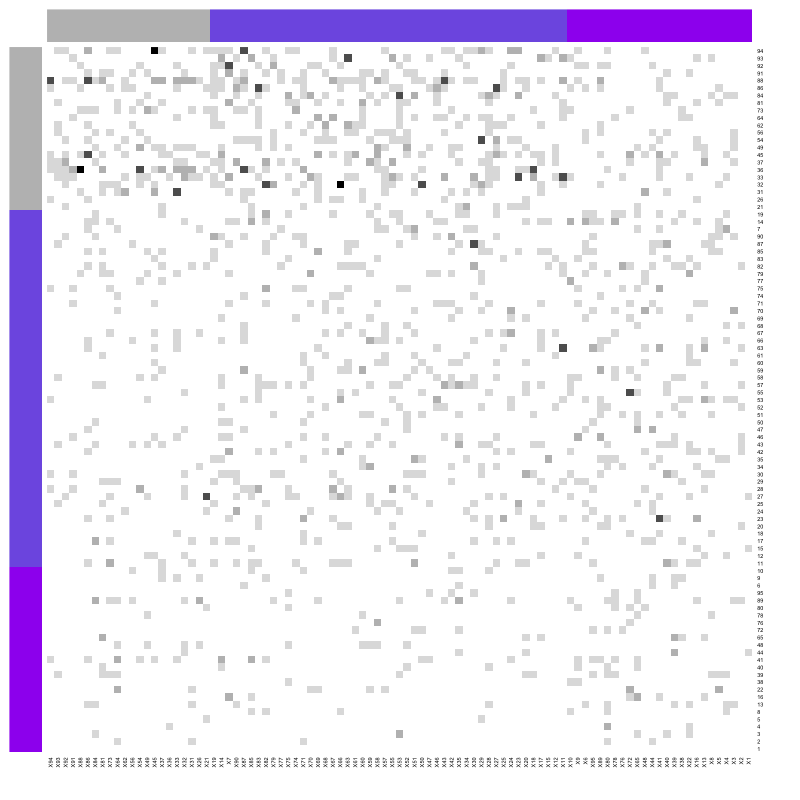
\includegraphics[width=.33\textwidth,natwidth=800,natheight=800]{/Users/lapo_santi/Desktop/Nial/POMM_pairwise/POMMs/Tennis application/results/processed_results/adjacency_Tennis_application_Est_model_POMM_K3_N95.png}%
        \label{fig:POMM_adjacency_K3}%
    }\hfill
    \subfigure[K=4, POMM Model]{%
        \includegraphics[width=.33\textwidth,natwidth=800,natheight=800]{/Users/lapo_santi/Desktop/Nial/POMM_pairwise/POMMs/Tennis application/results/processed_results/adjacency_Tennis_application_Est_model_POMM_K4_N95.png}%
        \label{fig:POMM_adjacency_K5}%
    }\hfill
    \subfigure[K=5 POMM Model]{%
        \includegraphics[width=.33\textwidth,natwidth=800,natheight=800]{/Users/lapo_santi/Desktop/Nial/POMM_pairwise/POMMs/Tennis application/results/processed_results/adjacency_Tennis_application_Est_model_POMM_K5_N95.png}%
        \label{fig:POMM_adjacency_K9}%
    }
    \caption{Adjacency Matrices simulated via the POMM Model}
    \label{fig:all_images}
\end{figure}



\begin{figure}[h]
    \centering
    \subfigure[K=3, Simple Model]{%
        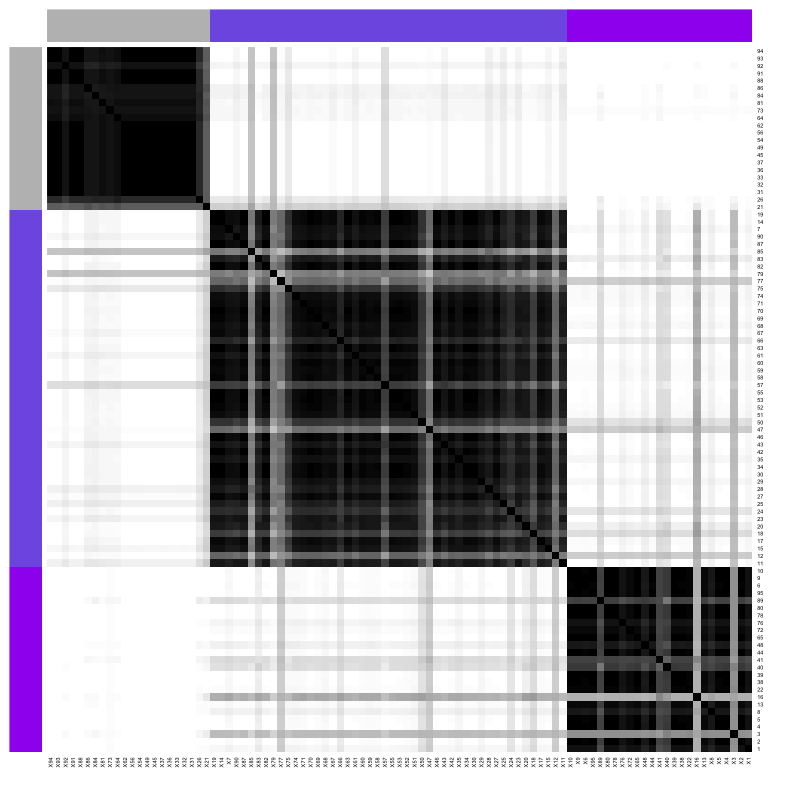
\includegraphics[width=.33\textwidth,natwidth=800,natheight=800]{/Users/lapo_santi/Desktop/Nial/POMM_pairwise/POMMs/Tennis application/results/processed_results/similarity_Tennis_application_Est_model_SimpleK3_N95.png}%
        \label{fig:POMM_adjacency_K3}%
    }\hfill
    \subfigure[K=4, Simple Model]{%
        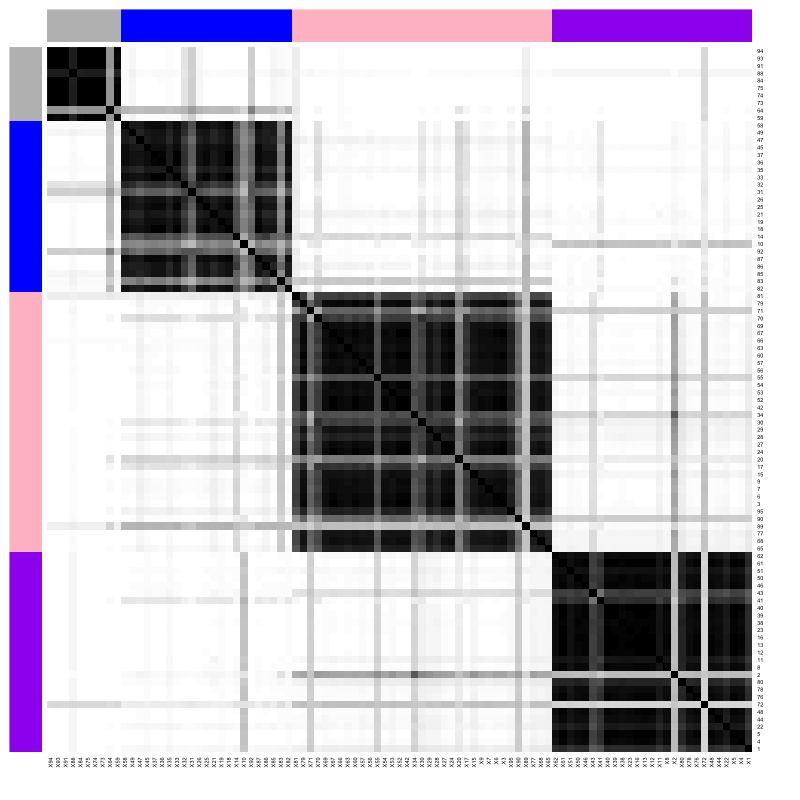
\includegraphics[width=.33\textwidth,natwidth=800,natheight=800]{/Users/lapo_santi/Desktop/Nial/POMM_pairwise/POMMs/Tennis application/results/processed_results/similarity_Tennis_application_Est_model_SimpleK4_N95.png}%
        \label{fig:POMM_adjacency_K5}%
    }\hfill
    \subfigure[K=5, Simple Model]{%
        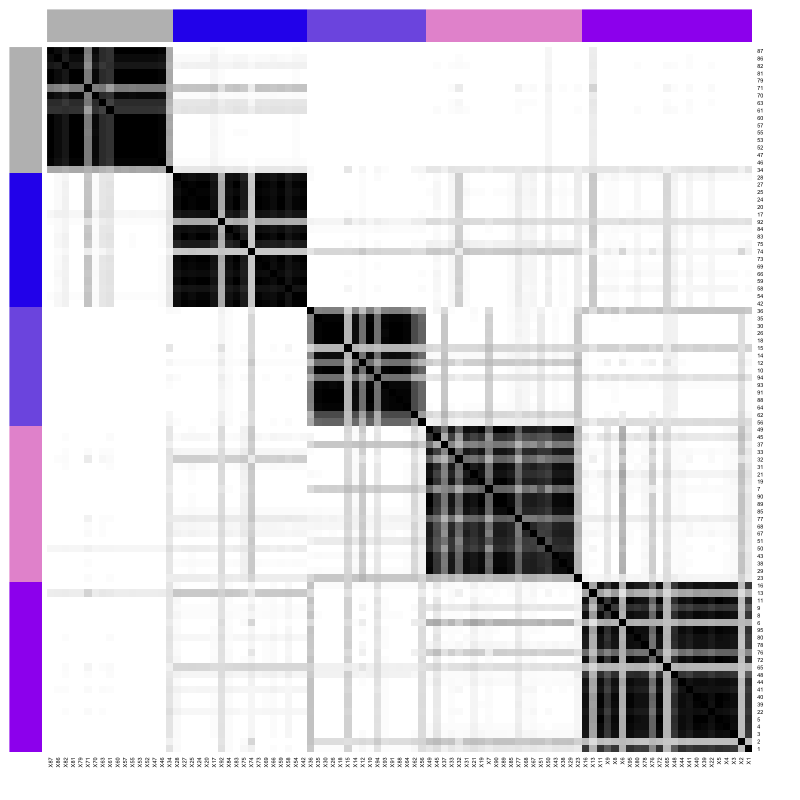
\includegraphics[width=.33\textwidth,natwidth=800,natheight=800]{/Users/lapo_santi/Desktop/Nial/POMM_pairwise/POMMs/Tennis application/results/processed_results/similarity_Tennis_application_Est_model_SimpleK5_N95.png}%
        \label{fig:POMM_adjacency_K9}%
    }\\[2ex]\subfigure[K=3, POMM Model]{%
        \includegraphics[width=.33\textwidth,natwidth=800,natheight=800]{/Users/lapo_santi/Desktop/Nial/POMM_pairwise/POMMs/Tennis application/results/processed_results/similarity_Tennis_application_Est_model_POMMK3_N95.png}%
        \label{fig:POMM_adjacency_K3}%
    }\hfill
    \subfigure[K=4, POMM Model]{%
        \includegraphics[width=.33\textwidth,natwidth=800,natheight=800]{/Users/lapo_santi/Desktop/Nial/POMM_pairwise/POMMs/Tennis application/results/processed_results/similarity_Tennis_application_Est_model_POMMK4_N95.png}%
        \label{fig:POMM_adjacency_K5}%
    }\hfill
    \subfigure[K=5 POMM Model]{%
        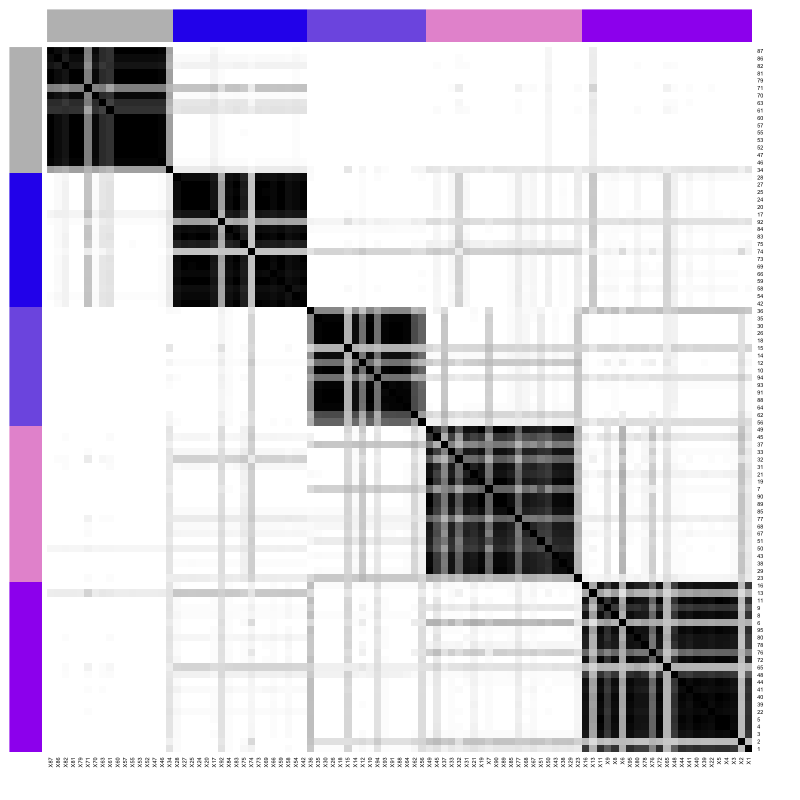
\includegraphics[width=.33\textwidth,natwidth=800,natheight=800]{/Users/lapo_santi/Desktop/Nial/POMM_pairwise/POMMs/Tennis application/results/processed_results/similarity_Tennis_application_Est_model_POMMK5_N95.png}%
        \label{fig:POMM_adjacency_K9}%
    }
    \caption{Adjacency Matrices simulated via the POMM Model}
    \label{fig:all_images}
\end{figure}


\begin{figure}[htbp]
    \centering
    \subfigure[K=3, Simple Model Estimates]{%
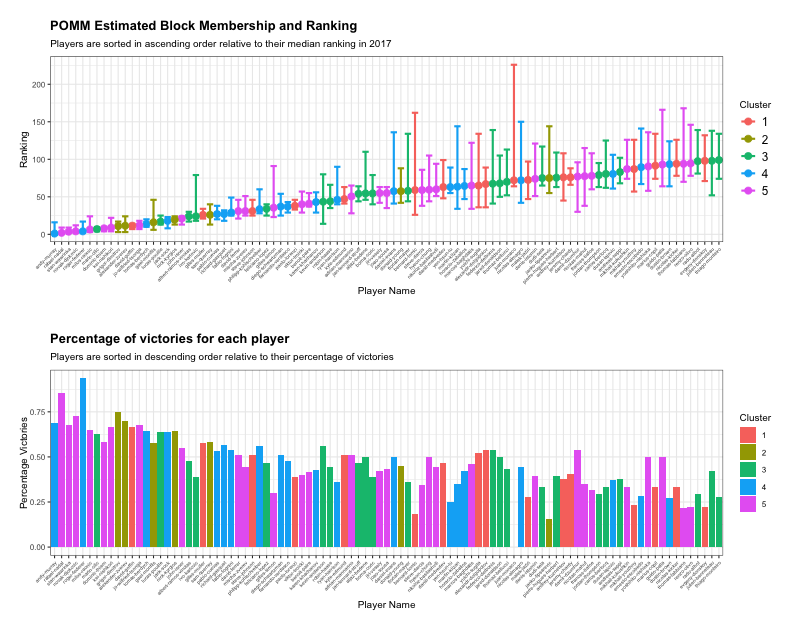
\includegraphics[width=.3333\textwidth,natwidth=800,natheight=800]{/Users/lapo_santi/Desktop/Nial/POMM_pairwise/POMMs/Tennis application/results/processed_results/RankvsClust_Est_modelSimple_K3_N95.png}%
        \label{fig:M4000}%
    }\hfill
    \subfigure[K=5, Simple Model Estimates]{%
        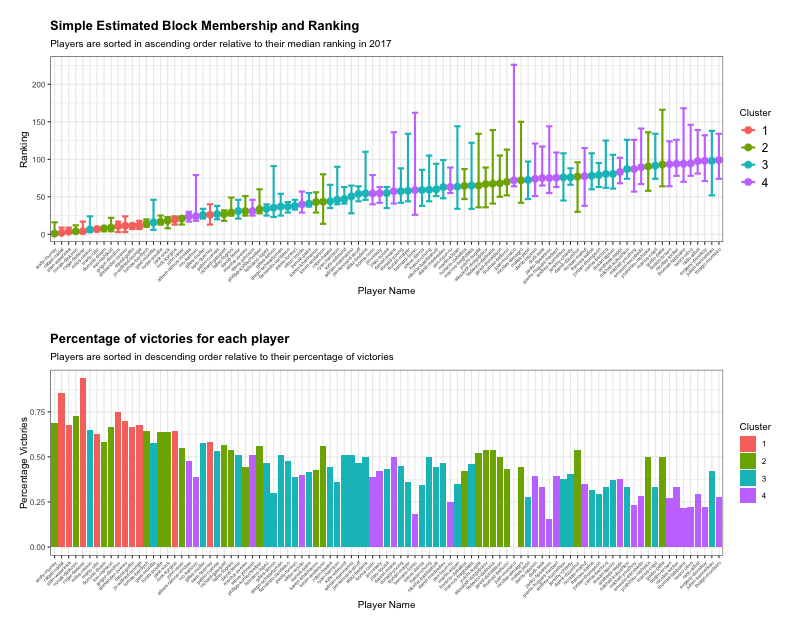
\includegraphics[width=.3333\textwidth,natwidth=800,natheight=800]{/Users/lapo_santi/Desktop/Nial/POMM_pairwise/POMMs/Tennis application/results/processed_results/RankvsClust_Est_modelSimple_K4_N95.png}%
        \label{fig:M7000}%
    }\hfill
    \subfigure[K=9, Simple Model Estimates]{%
        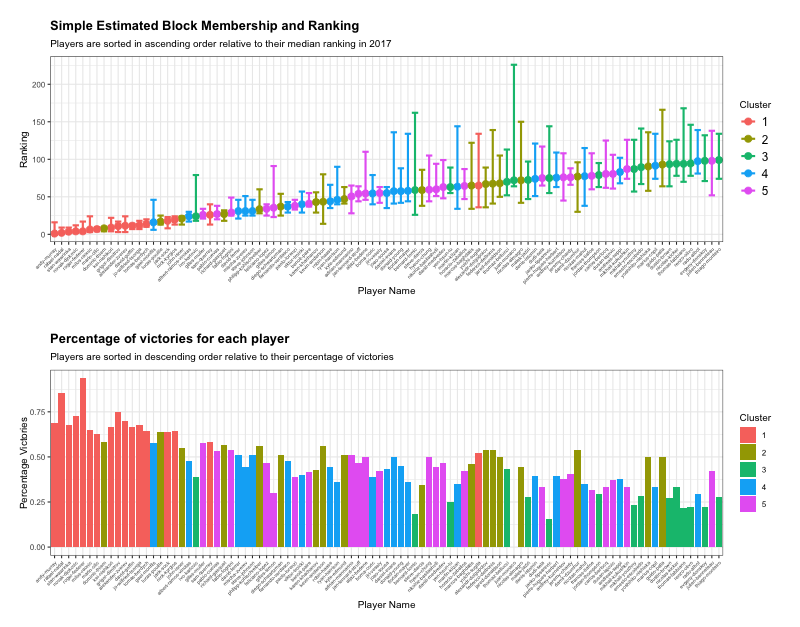
\includegraphics[width=.3333\textwidth,natwidth=800,natheight=800]{/Users/lapo_santi/Desktop/Nial/POMM_pairwise/POMMs/Tennis application/results/processed_results/RankvsClust_Est_modelSimple_K5_N95.png}%
        \label{fig:M10000}%
    }\\[2ex]\subfigure[K=3, POMM Model Estimates]{%
        \includegraphics[width=.3333\textwidth,natwidth=800,natheight=800]{/Users/lapo_santi/Desktop/Nial/POMM_pairwise/POMMs/Tennis application/results/processed_results/RankvsClust_Est_modelPOMM_K3_N95.png}%
        \label{fig:M4000}%
    }\hfill
    \subfigure[K=5, POMM Model Estimates]{%
\includegraphics[width=.3333\textwidth,natwidth=800,natheight=800]{/Users/lapo_santi/Desktop/Nial/POMM_pairwise/POMMs/Tennis application/results/processed_results/RankvsClust_Est_modelPOMM_K4_N95.png}%
        \label{fig:M7000}%
    }\hfill
    \subfigure[K=9, POMM Model Estimates]{%
        \includegraphics[width=.3333\textwidth,natwidth=800,natheight=800]{/Users/lapo_santi/Desktop/Nial/POMM_pairwise/POMMs/Tennis application/results/processed_results/RankvsClust_Est_modelPOMM_K5_N95.png}%
        \label{fig:M10000}%
    }
    \caption{Co-Clustering Matrices obtained via the Simple Model(above) and the POMM model (below).}
    \label{fig:all_images}
\end{figure}

 $$\hat{P}^{POMM}=\left[\begin{array}{ccc}
 0.500 & 0.779 & 0.648 \\
0.221 & 0.500 & 0.765 \\
0.352 & 0.235 & 0.500 
\end{array}\right] \quad \hat{P}^{Simple}=\left[\begin{array}{ccc}
0.500 & 0.779 & 0.648 \\
0.221 & 0.500 & 0.766 \\
0.352 & 0.234 & 0.500 
\end{array}\right]
$$

$$\hat{P}^{POMM}=\left[\begin{array}{cccc}0.500 & 0.786 & 0.742 & 0.764 \\
0.214 & 0.500 & 0.775 & 0.532 \\
0.258 & 0.225 & 0.500 & 0.776 \\
0.236 & 0.468 & 0.224 & 0.500 \end{array}\right] \quad \hat{P}^{Simple}=\left[\begin{array}{cccc}
0.500 & 0.787 & 0.742 & 0.763 \\
0.213 & 0.500 & 0.775 & 0.532 \\
0.258 & 0.225 & 0.500 & 0.775 \\
0.237 & 0.468 & 0.225 & 0.500 
 \end{array}\right]
$$

$$
\hat{P}^{POMM}= \left[\begin{array}{ccccc}0.500 & 0.778 & 0.745 & 0.785 & 0.716 \\
0.222 & 0.500 & 0.792 & 0.512 & 0.768 \\
0.255 & 0.208 & 0.500 & 0.747 & 0.652 \\
0.215 & 0.488 & 0.253 & 0.500 & 0.776 \\
0.284 & 0.232 & 0.348 & 0.224 & 0.500 \end{array}\right] \quad \hat{P}^{Simple}= \left[\begin{array}{ccccc}0.500 & 0.779 & 0.745 & 0.785 & 0.714 \\
0.221 & 0.500 & 0.792 & 0.512 & 0.768 \\
0.255 & 0.208 & 0.500 & 0.748 & 0.652 \\
0.215 & 0.488 & 0.252 & 0.500 & 0.777 \\
0.286 & 0.232 & 0.348 & 0.223 & 0.500 \end{array}\right]
$$





\begin{table}[htbp]
\centering
\caption*{
{\large $z$ summary table} \\ 
{\small True Model POMM, $N=100$}
} 
\begin{tabular}{cccc}
\toprule
\multirow{2}{*}{Method}  &\multicolumn{3}{c}{WAIC} \\
\cmidrule(lr){2-4}
& $(a)$ & $(b)$ & $(c)$  \\
\midrule
POMM model  &$\underset{24.85}{-5410.20}$ & $\underset{24.78}{-5536.49}$ & $\underset{25.51}{-5637.33}$  \\
Simple model  &$\underset{24.87}{-5411.18}$ & $\underset{24.76}{-5535.89}$ & $\underset{25.48}{-5637.28}$ \\
\bottomrule
\end{tabular}
\label{table:simulations_from_simple}
\end{table}


\begin{table}[htbp]
\centering
\caption*{
{\large POMM Hyperparameters summary table} \\ 
{\small True Model POMM, $N=100$}
} 
\begin{tabular}{ccccccc}
\toprule
\multirow{2}{*}{Method} & \multicolumn{3}{c}{
$\hat{\theta}$} & \multicolumn{3}{c}{
95$\%$ CI interval}  \\
\cmidrule(lr){2-4} \cmidrule(lr){5-7} 
& $(a)$ & $(b)$ & $(c)$ & $(a)$ & $(b)$ & $(c)$  \\
\midrule
$\Sigma$  &0.54 & 0.58 & 0.58 & [0.2	0.9] & [0.25	0.9] & [0.001,	0.0608]   \\
$\alpha$ & 0.45& 0.50& 0.42 & [0.11	0.84] & [0.15	0.88] & [0.1	0.82] \\
\bottomrule
\end{tabular}
\label{table:simulations_from_simple}
\end{table}


\subsection{POMM model check}



\begin{table}[htbp]
\centering
\caption*{
{\large $z$ diagnostic table} \\ 
{\small True Model POMM, $N=100$}
} 
\begin{tabular}{ccccccccccccc}
\toprule
\multirow{2}{*}{Fitted Model} & \multicolumn{3}{c}{ESS} & \multicolumn{3}{c}{
ACF$_{30}$} & \multicolumn{3}{c}{$\%$ accepted} & \multicolumn{3}{c}{Gelman-Rubin}\\
\cmidrule(lr){2-4} \cmidrule(lr){5-7} \cmidrule(lr){8-10} \cmidrule(lr){11-13} 
& $(a)$ & $(b)$ & $(c)$ & $(a)$ & $(b)$ & $(c)$ & $(a)$ & $(b)$ & $(c)$ & $(a)$ & $(b)$ & $(c)$ \\
\midrule
POMM &11458.19 & 8062.46 & 11734.00 & 0.14 & 0.13 & 0.06 & 1.76 & 1.15 & 0.94 & 1.01 & 1.01 & 1.01  \\
Simple &12846.46 & 8137.83 & 10373.67 & 0.10 & 0.18 & 0.05 & 1.63 & 1.17 & 0.92 & 1.01 & 1.07 & 1.01    \\
\bottomrule
\end{tabular}
\label{table:simulations_from_simple}
\end{table}

\begin{table}[htbp]
\centering
\caption*{
{\large $P$ diagnostic table} \\ 
{\small True Model POMM, $N=100$}
} 
\begin{tabular}{ccccccccccccc}
\toprule
\multirow{2}{*}{Fitted Model} & \multicolumn{3}{c}{ESS} & \multicolumn{3}{c}{
ACF$_{30}$} & \multicolumn{3}{c}{$\%$ accepted} & \multicolumn{3}{c}{Gelman-Rubin}\\
\cmidrule(lr){2-4} \cmidrule(lr){5-7} \cmidrule(lr){8-10} \cmidrule(lr){11-13} 
& $(a)$ & $(b)$ & $(c)$ & $(a)$ & $(b)$ & $(c)$ & $(a)$ & $(b)$ & $(c)$ & $(a)$ & $(b)$ & $(c)$ \\
\midrule
POMM &947.67 & 1414.33 & 2051.6 & 0.11 & 0.08 & 0.05 & 29.96 & 29.59 & 32.31 & 1 & 1.00 & 1 \\
Simple &1001.33 & 1365.83 & 1928.5 & 0.10 & 0.08 & 0.05 & 30.17 & 29.72 & 32.32 & 1 & 1.01 & 1\\
\bottomrule
\end{tabular}
\label{table:P_diagnostic_simple}
\end{table}


\begin{table}[htbp]
\centering
\caption*{
{\large POMM hyperparameters diagnostic table} \\ 
{\small True Model POMM, $N=100$}
} 
\begin{tabular}{ccccccccccccc}
\toprule
\multirow{2}{*}{Fitted Model} & \multicolumn{3}{c}{ESS} & \multicolumn{3}{c}{
ACF$_{30}$} & \multicolumn{3}{c}{$\%$ accepted} & \multicolumn{3}{c}{Gelman-Rubin}\\
\cmidrule(lr){2-4} \cmidrule(lr){5-7} \cmidrule(lr){8-10} \cmidrule(lr){11-13} 
& $(a)$ & $(b)$ & $(c)$ & $(a)$ & $(b)$ & $(c)$ & $(a)$ & $(b)$ & $(c)$ & $(a)$ & $(b)$ & $(c)$ \\
\midrule
$\Sigma$ &3504 & 4202 & 5078 & -0.01 & 0 & 0.01 & 37.25 & 34.56 & 34.16 & 1 & 1 & 1 \\
$\alpha$ &10 & 13 & 15 & 0.96 & 0.96 & 0.97 & 25.42 & 25.07 & 24.88 & 1.19 & 1.01 & 1.1     \\
\bottomrule
\end{tabular}
\label{table:simulations_from_simple}
\end{table}

\clearpage

\subsection{Fixing $\Sigma$=0.01}

\begin{figure}[htbp]
    \centering
    \subfigure[K=3, POMM Model Estimates]{%
\includegraphics[width=.3333\textwidth,natwidth=800,natheight=800]{/Users/lapo_santi/Desktop/Nial/POMM_pairwise/POMMs/Tennis application/fixing_S/processed_results/RankvsClust_Est_modelPOMM_K3_N95.png}%
        \label{fig:M4000}%
    }\hfill
    \subfigure[K=5, POMM Model Estimates]{%
        \includegraphics[width=.3333\textwidth,natwidth=800,natheight=800]{/Users/lapo_santi/Desktop/Nial/POMM_pairwise/POMMs/Tennis application/fixing_S/processed_results/RankvsClust_Est_modelPOMM_K4_N95.png}%
        \label{fig:M7000}%
    }\hfill
    \subfigure[K=9, POMM Model Estimates]{%
    \includegraphics[width=.3333\textwidth,natwidth=800,natheight=800]{/Users/lapo_santi/Desktop/Nial/POMM_pairwise/POMMs/Tennis application/fixing_S/processed_results/RankvsClust_Est_modelPOMM_K5_N95.png}%
        \label{fig:M10000}%
    }
    \end{figure}


$$\hat{P}^{POMM}=\left[\begin{array}{ccc}
0.50& 0.65 & 0.79\\
0.34& 0.50 & 0.64 \\
0.21& 0.35 & 0.50
\end{array}\right]
$$

$$\hat{P}^{POMM}=\left[\begin{array}{cccc}
0.50 & 0.58 & 0.68 & 0.76 \\
0.42 & 0.50 & 0.57 & 0.67 \\
0.32 & 0.43 & 0.50 & 0.57 \\
0.24 & 0.33 & 0.43 & 0.50 \end{array}\right] 
$$

$$
\hat{P}^{POMM}= \left[\begin{array}{ccccc}
0.50 & 0.58 & 0.67 & 0.72 & 0.79 \\
0.42 & 0.50 & 0.57 & 0.67 & 0.71 \\
0.33 & 0.43 & 0.50 & 0.57 & 0.67 \\
0.28 & 0.33 & 0.43 & 0.50 & 0.58 \\
0.22 & 0.29 & 0.33 & 0.42 & 0.50\end{array}\right]
$$



\begin{figure}[h]
    \centering
    \subfigure[K=3, Simple Model]{%
        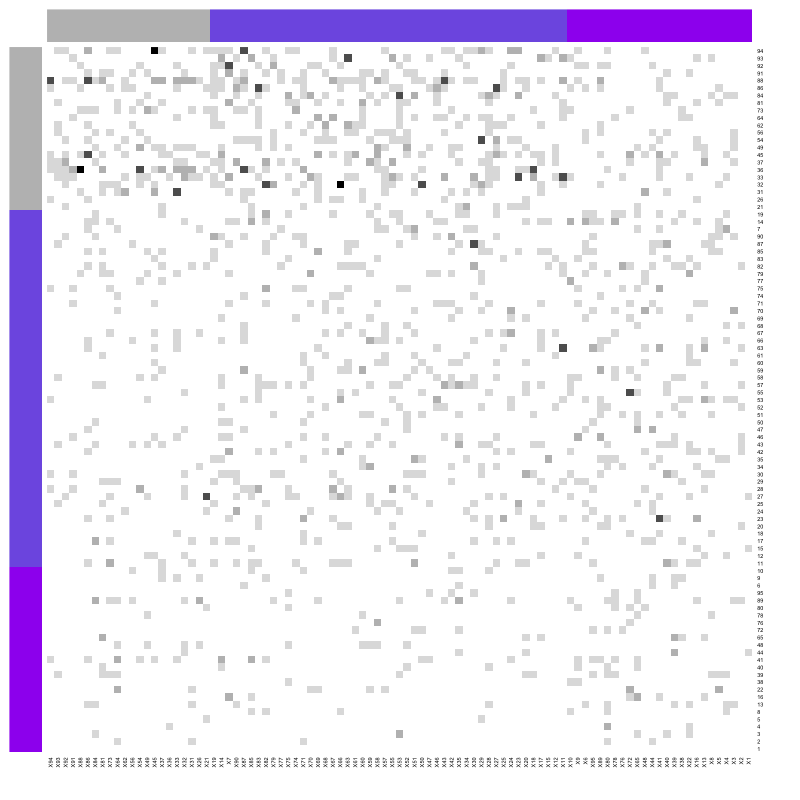
\includegraphics[width=.33\textwidth,natwidth=800,natheight=800]{/Users/lapo_santi/Desktop/Nial/POMM_pairwise/POMMs/Tennis application/results/processed_results/adjacency_Tennis_application_Est_model_POMM_K3_N95.png}%
        \label{fig:POMM_adjacency_K3}%
    }\hfill
    \subfigure[K=4, Simple Model]{%
        \includegraphics[width=.33\textwidth,natwidth=800,natheight=800]{/Users/lapo_santi/Desktop/Nial/POMM_pairwise/POMMs/Tennis application/fixing_S/processed_results/adjacency_Tennis_application_Est_model_POMM_K4_N95.png}%
        \label{fig:POMM_adjacency_K5}%
    }\hfill
    \subfigure[K=5, Simple Model]{%
        \includegraphics[width=.33\textwidth,natwidth=800,natheight=800]{/Users/lapo_santi/Desktop/Nial/POMM_pairwise/POMMs/Tennis application/fixing_S/processed_results/adjacency_Tennis_application_Est_model_POMM_K5_N95.png}%
        \label{fig:POMM_adjacency_K9}%
    }\\[2ex]\subfigure[K=3, POMM Model]{%
        \includegraphics[width=.33\textwidth,natwidth=800,natheight=800]{/Users/lapo_santi/Desktop/Nial/POMM_pairwise/POMMs/Tennis application/fixing_S/processed_results/similarity_Tennis_application_Est_model_POMMK3_N95.png}%
        \label{fig:POMM_adjacency_K3}%
    }\hfill
    \subfigure[K=4, POMM Model]{%
        \includegraphics[width=.33\textwidth,natwidth=800,natheight=800]{/Users/lapo_santi/Desktop/Nial/POMM_pairwise/POMMs/Tennis application/fixing_S/processed_results/similarity_Tennis_application_Est_model_POMMK4_N95.png}%
        \label{fig:POMM_adjacency_K5}%
    }\hfill
    \subfigure[K=5 POMM Model]{%
        \includegraphics[width=.33\textwidth,natwidth=800,natheight=800]{/Users/lapo_santi/Desktop/Nial/POMM_pairwise/POMMs/Tennis application/fixing_S/processed_results/similarity_Tennis_application_Est_model_POMMK5_N95.png}%
        \label{fig:POMM_adjacency_K9}%
    }
    \caption{Adjacency Matrices simulated via the POMM Model}
    \label{fig:all_images}
\end{figure}

\begin{table}[htbp]
\centering
\caption*{
{\large $z$ summary table} \\ 
{\small True Model POMM, $N=100$}
} 
\begin{tabular}{cccc}
\toprule
\multirow{2}{*}{Method}  &\multicolumn{3}{c}{WAIC} \\
\cmidrule(lr){2-4}
& $(a)$ & $(b)$ & $(c)$  \\
\midrule
POMM model  &$\underset{21.17}{-5220.111}$ & $\underset{19.32}{-5181.395}$ & $\underset{20.07}{-5233.632}$  \\  
\bottomrule
\end{tabular}
\label{table:simulations_from_simple}
\end{table}


\begin{table}[htbp]
\centering
\caption*{
{\large POMM Hyperparameters summary table} \\ 
{\small True Model POMM, $N=100$}
} 
\begin{tabular}{ccccccc}
\toprule
\multirow{2}{*}{Method} & \multicolumn{3}{c}{
$\hat{\theta}$} & \multicolumn{3}{c}{
95$\%$ CI interval}  \\
\cmidrule(lr){2-4} \cmidrule(lr){5-7} 
& $(a)$ & $(b)$ & $(c)$ & $(a)$ & $(b)$ & $(c)$  \\
\midrule
$\Sigma$ &0.01 & 0.01 & 0.01 & [0.01	0.01] & [0.01	0.01] & [0.01	0.01]   \\
$\alpha$ & 0.12 & 1.41 & 0.87 & [0.1	0.15] & [0.1	2.74] & [0.1	1.8] \\
\bottomrule
\end{tabular}
\label{table:simulations_from_simple}
\end{table}








\begin{table}[htbp]
\centering
\caption*{
{\large $z$ diagnostic table} \\ 
{\small True Model POMM, $N=100$}
} 
\begin{tabular}{ccccccccccccc}
\toprule
\multirow{2}{*}{Fitted Model} & \multicolumn{3}{c}{ESS} & \multicolumn{3}{c}{
ACF$_{30}$} & \multicolumn{3}{c}{$\%$ accepted} & \multicolumn{3}{c}{Gelman-Rubin}\\
\cmidrule(lr){2-4} \cmidrule(lr){5-7} \cmidrule(lr){8-10} \cmidrule(lr){11-13} 
& $(a)$ & $(b)$ & $(c)$ & $(a)$ & $(b)$ & $(c)$ & $(a)$ & $(b)$ & $(c)$ & $(a)$ & $(b)$ & $(c)$ \\
\midrule
POMM &29353.04 & 20673.88 & 23681.54 & 0 & 0 & 0.01 & 8.93 & 15.05  & 16.53 & 1 & 1.13 & 1.16    \\
\bottomrule
\end{tabular}
\label{table:simulations_from_simple}
\end{table}

\begin{table}[htbp]
\centering
\caption*{
{\large $P$ diagnostic table} \\ 
{\small True Model POMM, $N=100$}
} 
\begin{tabular}{ccccccccccccc}
\toprule
\multirow{2}{*}{Fitted Model} & \multicolumn{3}{c}{ESS} & \multicolumn{3}{c}{
ACF$_{30}$} & \multicolumn{3}{c}{$\%$ accepted} & \multicolumn{3}{c}{Gelman-Rubin}\\
\cmidrule(lr){2-4} \cmidrule(lr){5-7} \cmidrule(lr){8-10} \cmidrule(lr){11-13} 
& $(a)$ & $(b)$ & $(c)$ & $(a)$ & $(b)$ & $(c)$ & $(a)$ & $(b)$ & $(c)$ & $(a)$ & $(b)$ & $(c)$ \\
\midrule
POMM &2018.33 & 1900 & 2983.4 & 0.01 & 0.02 & 0.01 & 33.8 & 27.57 & 29.75 & 1 & 12.35 & 10.89  \\
\bottomrule
\end{tabular}
\label{table:simulations_from_simple}
\end{table}

\clearpage

\subsubsection{Montecarlo algorithm}




First, it should be noted that within the same block we observe a substantial variability. We may have players that win against other players of the same cluster, against players of weaker clusters, or that simply do not win much. If we have players that substantially win against players of stronger clusters, it means that they are misclassified. So the fundamental variability driver is to be recognised in the blocks of the defeated players. Winning against Federer is not the same as winning against a newcomer. Those two victories should not be accounted in the same fashion.

However, one could argue that if the block exhibits a large amount of variability, this probably means that we should split the block further in two, to possibly account for different patterns of victories.

Another crucial point is data imbalance. Games are not drawn at random, which means that we will observe strongest player playing more with each other, since they are the on remaining within the tournament for longer periods, and weaker players playing less against the strong ones and more among themselves.

The issue is that by assigning one cluster to a player is equivalent to equip them with a single probability to beat all the players within a given cluster.







\begin{comment}

\begin{comment}

\section{ATP tennis dataset}


Our raw data are in a repository which can be found at \begin{center}\texttt{'https://pkgstore.datahub.io/sports-data/atp-world-tour-tennis-data'}\end{center}. If two players have played multiple times, they compare on different rows as we can see in Table(1). 

\begin{table}
\begin{center}\begin{tabular}{cccc} $\textbf{Winner}$ & $\textbf{Loser}$ \\Djockovic & Medvedev \\ \vdots & \vdots \\Djockovic & Medvedev  \\Djockovic & Medvedev \\ Medvedev & Djockovic \\\vdots & \vdots \\ Medvedev & Djockovic \\ Medvedev & Djockovic  \end{tabular} \caption{Raw data}
\end{center}
\label{Raw data}
\end{table}

To begin with, we select all rows with the first pair of players, regardless of the order in which they appear. Then, we construct these two new variables:
\begin{itemize}
\item $n_{games}$: the total number of games between player A and player B, which can be calculated as the sum of the number of victories of player A against player B and the number of victories of player B against player A. Basically, one counts the number of times these two names appear on the same row, irrespective of their order.
\item $n_{victories}$: the total number of victories of player A against player B, which can be calculated as the number of times player A appears before player B on the same row.
\end{itemize}

Then, I retain just the first pair observation, e.g. player A and player B, and disregard all the others. This process is repeated for all unique unordered pairs of players. In this way, I obtain a dataset storing, for each pair of players who have played at least once, all the relevant information in one single entry.

What about the observations in which player B won against player A? These will no longer be entries in the dataframe. However, this data will still be indirectly available by computing the total number of games between player A and player B (available in column $n_{games}$, at the corresponding row) minus the total number of victories of player A against player B (available in $n_{victories}$, at the corresponding row).

The final dataframe will look like as in Table (2).
\begin{table}
\begin{center}\begin{tabular}{cccc} $\textbf{Player1}$ & $\textbf{Player2}$ & $n_{games}$ & $n_{victories}$ \\Djockovic & Medvedev & 5 & 3 \\Djockovic & Nadal & 8 & 6 \\Nadal & Tsonga & 4 & 0\end{tabular} \caption{Final dataset}
\end{center}
\label{Final dataset}
\end{table}

\clearpage









\section{Descriptive statistics comparing simulated vs ATP data}


We start by choosing a particular configuration of parameters to simulate a given tournament to compare it with the ATP data.
\begin{itemize}
\item \texttt{N}=537 since in the ATP dataset we have exactly 537 players
\item \texttt{M}=3389 since in the ATP dataset this is the total number of matches
\item \texttt{max\_number\_games} = 4 since this is the max value we observe in the ATP data.
\end{itemize}
So, for these three initial parameters, we are replicating the features of the real tennis data. With respect to the more "statistical" ones there is no benchmark, so we choose to follow the intuition:
\begin{itemize}
\item \texttt{max\_clust}=3
\item \texttt{min\_clust}=3
\item \texttt{c} = 1.7
\item \texttt{beta\_max} = .8
\end{itemize}
After generating the data, we compare the simulated tournament and the true ATP data by computing some summary statistics and some meaningful plots shown in Figures (\ref{fig:scatterplot}), (\ref{fig:boxplotnij}), (\ref{fig:densityplotnij}), (\ref{fig:boxplotyij}), (\ref{fig:densityplotyij}). The scatterplot shows a similar pattern of strong correlation between $y_{ij}$ and $n_{ij}$. However, in ATP there is a higher points density close to the origin, while in the simulated tournament we have more density close to the mean. It means that real data are more dispersed than simulated ones. We can reach the same conclusion by looking at the number of games distribution and the number of victories. In particular, by looking at Figures (\ref{fig:boxplotyij}) and (\ref{fig:densityplotyij}) the discrepancy seems more enhanced for the number of victories $y_{ij}$. 

The interesting aspect of this methodology is that we could compute the discrepancy between the two distributions, for example using a Kullback-Leibler divergence, and find those parameters that minimize it.

\begin{figure}
\begin{minipage}{.8\textwidth}
      \centering
\includegraphics[width=.5\textwidth,natwidth=400,natheight=330]{/Users/lapo_santi/Desktop/Nial/project/descriptive statistic/comparison statistics/Scatterplot.png}
\caption{Scatterplot of $n_{ij}$, the number of games played between any two pair of players, and $y_{ij}$, the number of victories of player $i$ vs player $j$. We show the values both for Simulated (blue) and ATP data (red)}
\label{fig:scatterplot}
\end{minipage}\hfill
    \centering
    \begin{minipage}{0.25\textwidth}
        \centering
\includegraphics[width=\textwidth,natwidth=400,natheight=330]{/Users/lapo_santi/Desktop/Nial/project/descriptive statistic/comparison statistics/boxplotnij.png}
        \caption{Boxplot of $n_{ij}$ values both for Simulated (blue) and ATP data (red)}
        \label{fig:boxplotnij}
    \end{minipage}
    \begin{minipage}{0.25\textwidth}
        \centering
        \includegraphics[width=\textwidth,natwidth=400,natheight=330]{/Users/lapo_santi/Desktop/Nial/project/descriptive statistic/comparison statistics/densityplotnij.png}
        \caption{Density Plot for the $n_{ij}$ values both for Simulated (blue) and ATP data (red)}
        \label{fig:densityplotnij}
    \end{minipage}
    \vskip\floatsep
    \begin{minipage}{0.25\textwidth}
        \centering
 \includegraphics[width=\textwidth,natwidth=400,natheight=330]{/Users/lapo_santi/Desktop/Nial/project/descriptive statistic/comparison statistics/boxplotyij.png}
        \caption{Boxplot of $y_{ij}$ values both for Simulated (blue) and ATP data (red)}
        \label{fig:boxplotyij}
    \end{minipage}
    \begin{minipage}{0.25\textwidth}
        \centering
        \includegraphics[width=\textwidth,natwidth=400,natheight=330]{/Users/lapo_santi/Desktop/Nial/project/descriptive statistic/comparison statistics/densityplotyij.png}
        \caption{Density Plot for the $n_{ij}$ values both for Simulated (blue) and ATP data (red)}
        \label{fig:densityplotyij}
    \end{minipage}
\end{figure}



\end{comment}







\clearpage

\section{Appendix I: Estimation Details}


\subsection{Updating z}

To update $z$ we propose a new label for each node, we evaluate the accept/reject move by computing the ratio $r$ as follows:
\begin{align}
r &= \frac{\prod_{i<j}\binom{n_{ij}}{y_{ij}}p_{z^{\prime}_i z^{\prime}_j}^{y_{ij}} \cdot (1 - p_{z^{\prime}_i z^{\prime}_j})^{n_{ij} - y_{ij}} \cdot \frac{\Gamma(\gamma_0) \Gamma(n+1)}{\Gamma(n + \gamma_0)} \cdot \prod_{k=1}^K \frac{\Gamma(n^{\prime}_k + \gamma_k)}{\Gamma(\gamma_k)  \Gamma(n^{\prime}_k + 1)}}{\prod_{i<j}\binom{n_{ij}}{y_{ij}}p_{z_iz_j}^{y_{ij}} \cdot (1 - p_{z_iz_j})^{n_{ij} - y_{ij}}\cdot \frac{\Gamma(\gamma_0) \Gamma(n+1)}{\Gamma(n + \gamma_0)} \cdot \prod_{k=1}^K \frac{\Gamma(n_k + \gamma_k)}{\Gamma(\gamma_k)  \Gamma(n_k + 1)}} \\
 &= \frac{\prod_{i<j}p_{z^{\prime}_i z^{\prime}_j}^{y_{ij}} \cdot (1 - p_{z^{\prime}_i z^{\prime}_j})^{n_{ij} - y_{ij}} \cdot  \prod_{k=1}^K \frac{\Gamma(n^{\prime}_k + \gamma_k)}{\Gamma(\gamma_k)  \Gamma(n^{\prime}_k + 1)}}{\prod_{i<j}p_{z_iz_j}^{y_{ij}} \cdot (1 - p_{z_iz_j})^{n_{ij} - y_{ij}} \cdot \prod_{k=1}^K \frac{\Gamma(n_k + \gamma_k)}{\Gamma(\gamma_k)  \Gamma(n_k + 1)}} 
\end{align}


Passing to the log:

\begin{align}
log(r) &= \log{ \left( \prod_{i<j}p_{z^{\prime}_i z^{\prime}_j}^{y_{ij}} \cdot (1 - p_{z^{\prime}_i z^{\prime}_j})^{n_{ij} - y_{ij}} \cdot  \prod_{k=1}^K \frac{\Gamma(n^{\prime}_k + \gamma_k)}{\Gamma(\gamma_k)  \Gamma(n^{\prime}_k + 1)} \right) }  \nonumber \\
& \qquad - \log{ \left( \prod_{i<j}p_{z_iz_j}^{y_{ij}} \cdot (1 - p_{z_iz_j})^{n_{ij} - y_{ij}} \cdot \prod_{k=1}^K \frac{\Gamma(n_k + \gamma_k)}{\Gamma(\gamma_k)  \Gamma(n_k + 1)}\right)} \nonumber \\
&= \sum_{i<j} \left(   y_{ij} \cdot \log{ p_{z^{\prime}_i z^{\prime}_j} } + (n_{ij} - y_{ij}) \cdot \log{ (1 - p_{z^{\prime}_i z^{\prime}_j}) } \right)\nonumber \\ 
&\qquad +  \sum_{k=1}^K\left(\log\left(\Gamma(n^{\prime}_{k}+\gamma_{k})\right) - \log\left(\Gamma(\gamma_{k})\right) - \log\left(\Gamma\left(n^{\prime}_{k}+1\right)\right) \right)  \nonumber  \\
& \qquad \qquad - \sum_{i<j} \left(  y_{ij} \cdot \log{ p_{z_i z_j} } + (n_{ij} - y_{ij}) \cdot \log{ (1 - p_{z_i z_j}) } \right) \nonumber \\
&\qquad \qquad \qquad - \sum_{k=1}^K\left(\log\left(\Gamma(n_{k}+\gamma_{k})\right) - \log\left(\Gamma(\gamma_{k})\right) - \log\left(\Gamma\left(n_{k}+1\right)\right) \right) \nonumber \\
\end{align}


\begin{algorithm}
\begin{algorithmic}[1]
\For{$i \gets 1$ to $N$}
\State Sample $\texttt{new\_label}$ from $1,...,K$
\State Set $z^{\prime} \gets z$ with the $i$-th element replaced by $\texttt{new\_label}$
\State Compute new victory probabilities $p_{z^{\prime}_i z^{\prime}_j}$ using $z^{\prime}$
\State Compute probability ratio $log(r)$  using $p_{z^{\prime}_i z^{\prime}_j}$ and $p_{z_i z_j}$
\State Set $\alpha_{r} \gets \min(1, r)$
\State Sample $u$ from a uniform distribution on $(0,1)$
\If{$u < \alpha_{r}$}
\State Update $z$ to $z^{\prime}$
\State Update $p_{z_iz_j}$ to $p_{z^{\prime}_i z^{\prime}_j}$
\State Increment $acc.count_{z}$
\EndIf
\State Store $z_{current}$ in $z.container$
\EndFor
\end{algorithmic}
\label{alg:z_update}
\caption{Updating $z$ step}
\end{algorithm}


\subsection{Updating $\mathbf{P}$}


To update $P$ and $\alpha$ we propose a new label for each node, we evaluate the accept/reject move by computing the ratio $r$ as follows:

\begin{align}
r &= \frac{\prod_{i<j}\binom{n_{ij}}{y_{ij}}p_{z_i z_j}^{\prime y_{ij}} \cdot (1 - p^{\prime}_{z_i z_j})^{n_{ij} - y_{ij}} \cdot \prod_{k=1}^K  \left( \frac{1}{y^{\prime (k+1)} - y^{\prime(k)}}\right)^{|L^{\prime(k)}|}}{\prod_{i<j}\binom{n_{ij}}{y_{ij}}p_{z_i z_j}^{y_{ij}} \cdot (1 - p_{z_i z_j})^{n_{ij} - y_{ij}} \cdot \prod_{k=1}^K  \left( \frac{1}{y^{(k+1)} - y^{(k)}}\right)^{|L^{(k)}|}} \\
\end{align}


Passing to the log:

\begin{align}
log(r) &= \sum_{i<j} \left(  y_{ij} \cdot \log{ p^{\prime}_{z_i z_j} } + (n_{ij} - y_{ij}) \cdot \log{ (1 - p^{\prime}_{z_i z_j}) } \right)  - \sum_{k=1}^K |L^{\prime(k)}| \cdot \log{\left( y^{\prime(k+1)} - y^{\prime(k)} \right)}\\
 &\qquad - \sum_{i<j} \left(  y_{ij} \cdot \log{ p_{z_i z_j} } + (n_{ij} - y_{ij}) \cdot \log{ (1 - p_{z_i z_j}) } \right)  + \sum_{k=1}^K |L^{(k)}| \cdot \log{\left( y^{(k+1)} - y^{(k)} \right) }
\end{align}







\begin{algorithm}
\begin{algorithmic}[1]
\State $j \gets 1$
\While{$j \leq N_{iter}$}
\State Sample $\alpha^{\prime}$ from a truncated normal distribution
\State Generate a new proposal matrix $P^{\prime}$
\State Compute new victory probabilities $p_{z_iz_j}^{\prime}$ using $P^{\prime}$ and $z_{current}$
\State Compute probability ratio $log(r)$ using $p_{z_iz_j}^{\prime}$ and $p_{z_iz_j}$
\State Set $\alpha_{r} \gets \min(1, r)$
\State Sample $u$ from a uniform distribution on $(0,1)$
\If{$u < \alpha_{r}$}
\State Update $\alpha$ to $\alpha^{\prime}$
\State Update $P$ to $P^{\prime}$
\State Update $p_{z_iz_j}$ to $p_{z_iz_j}^{\prime}$
\State Increment $acc.count_{p}$
\EndIf
\State Store $P$ in $P.container$
\State Store $\alpha$ in $\alpha.container$

\State $j \gets j+1$
\EndWhile
\end{algorithmic}
\label{alg:P_update}
\caption{Updating $P$ step}
\end{algorithm}

\section{Appendix II: POMM prior checks}

\subsection{Prior predictive check}

\subsection{MLE check}


\begin{comment}

\section{Idea about a Gibbs sampler}

To derive the full conditional distribution of $\textbf{z}$ given the data $y$ and the hyperparameters $\boldsymbol{\gamma}$, we can use Bayes' theorem and write:

\begin{align*}
p(\textbf{z}|y,\boldsymbol{\gamma}) &\propto p(y|\textbf{z}) p(\textbf{z}|\boldsymbol{\gamma}) \
&\propto \prod_{i=1}^n \prod_{j=i+1}^n {n_{ij} \choose y_{ij}} (p_{z_i,z_j})^{y_{ij}} (1-p_{z_i,z_j})^{n_{ij}-y_{ij}} \prod_{k=1}^K \frac{\Gamma(\gamma_k + m_k)}{\Gamma(\gamma_k)}
\end{align*}

where we have dropped constant terms that do not depend on $\textbf{z}$. We can simplify this expression by collecting terms that depend on each $z_i$. Specifically, we can group the terms in the likelihood that involve $z_i$ with the prior probability of $z_i$ to get:

\begin{align*}
p(z_i|y,\textbf{z}{-i},\boldsymbol{\gamma}) &\propto p(y{i,\cdot}|\textbf{z}) p(z_i|\boldsymbol{\gamma}) \
&= \prod_{j\neq i} {n_{ij} \choose y_{ij}} (p_{z_i,z_j})^{y_{ij}} (1-p_{z_i,z_j})^{n_{ij}-y_{ij}} \frac{\Gamma(\gamma_{z_i} + m_{z_i})}{\Gamma(\gamma_{z_i})}
\end{align*}

where $\textbf{z}{-i}$ denotes all elements of $\textbf{z}$ except for $z_i$, and $y{i,\cdot}$ denotes the $i$th row of the $n\times n$ matrix of observations $y$. We can recognize the above expression as the likelihood of $z_i$ being drawn from a categorical distribution with parameter vector $\boldsymbol{\theta}{-i}$, where $\theta{k,-i} \propto \prod_{j\neq i} (p_{k,z_j})^{y_{ij}} (1-p_{k,z_j})^{n_{ij}-y_{ij}} \frac{\Gamma(\gamma_k + m_k)}{\Gamma(\gamma_k)}$ is the partial likelihood of $z_i$ being assigned value $k$, with $z_j$ for $j\neq i$ fixed to their current values. Thus, we have:

\begin{align*}
p(z_i=k|y,\textbf{z}{-i},\boldsymbol{\gamma}) &= \frac{\theta{k,-i}}{\sum_{k'} \theta_{k',-i}}
\end{align*}

for each possible value of $k$. This gives the full conditional distribution of $z_i$ given the data, the other $z_j$'s, and the hyperparameters.


\section{Possible applications}
The POMM model can have various applications in fields where pairwise comparisons are made. Some examples of applications are:
\begin{itemize}
\item Sports Analytics: The POMM model can be used to rank sports teams based on their pairwise comparison results. It can also be used to predict the probability of a team winning a match against another team.

\item Marketing: The POMM model can be used to rank products based on their pairwise comparison results in surveys. It can also be used to estimate the probability of a customer preferring one product over another.

\item Decision Making: The POMM model can be used to rank options based on their pairwise comparison results. It can also be used to estimate the probability of one option being preferred over another in a decision-making process.

\item Social Science: The POMM model can be used to study social preferences by asking individuals to compare two different options. For example, it can be used to understand people's preferences for different political candidates, policies, or social norms.

\item Biology: The POMM model can be used to study the relative fitness of different genotypes in evolutionary biology or the preferences of animals for different stimuli in behavioral ecology.
\end{itemize}
Overall, the POMM model can be applied in any field where pairwise comparisons are made and where the goal is to rank or estimate the probabilities of different options.



\begin{align}\log \left(\Pr(\mathbf{x}\mid n, \boldsymbol{\alpha})\right) &= \log\left(\frac{\Gamma\left(\alpha_0\right)\Gamma\left(n+1\right)}
{\Gamma\left(n+\alpha_0\right)}\prod_{k=1}^K\frac{\Gamma(x_{k}+\alpha_{k})}{\Gamma(\alpha_{k})\Gamma\left(x_{k}+1\right)}\right) \\
 &= \log\left(\Gamma\left(\alpha_0\right)\right) + \log\left(\Gamma\left(n+1\right)\right) - \log\left(\Gamma\left(n+\alpha_0\right)\right) \\ 
 & \qquad + \sum_{k=1}^K\left[\log\left(\Gamma(x_{k}+\alpha_{k})\right) - \log\left(\Gamma(\alpha_{k})\right) - \log\left(\Gamma\left(x_{k}+1\right)\right)\right] \end{align}

\end{comment}




\end{document}